\documentclass[a4paper,11pt]{article}
\usepackage[utf8]{inputenc}
\usepackage[T1]{fontenc}
\usepackage[spanish,es-tabla,es-nodecimaldot]{babel}
\usepackage[left=2.2cm, right=2.2cm, top=2.5cm, bottom=2.5cm, headheight=40pt]{geometry}
\usepackage{graphicx}
\usepackage{xcolor}
\usepackage{tabularx}
\usepackage{longtable}
\usepackage{etoolbox}
\usepackage{array}
\usepackage{booktabs}
\usepackage{colortbl}
\usepackage{fancyhdr}
\usepackage{titlesec}
\usepackage{enumitem}
\usepackage{microtype}
\usepackage{eso-pic}
\usepackage[sc, osf]{mathpazo}
\linespread{1.06}
\usepackage[scaled=.95,type1]{cabin}
\usepackage{inconsolata}
\usepackage{setspace}
\usepackage{tcolorbox}
\tcbuselibrary{skins,breakable}

\makeatletter
\patchcmd{\LT@output}{\copy\LT@foot\vss}{\copy\LT@foot\vskip 0pt plus \maxdimen minus \normalbaselineskip}{}{\PackageError{PROPUESTA_TECNICA}{No se pudo ajustar el espaciado de longtable}{}}
\patchcmd{\LT@output}{\copy\LT@foot\vss}{\copy\LT@foot\vskip 0pt plus \maxdimen minus \normalbaselineskip}{}{\PackageError{PROPUESTA_TECNICA}{No se pudo ajustar el espaciado de longtable}{}}
\makeatother

\usepackage[hyperfootnotes=false,colorlinks=true,linkcolor=clenchCyanDark,urlcolor=clenchCyanDark,citecolor=clenchCyanDark]{hyperref}

% Paleta visual de CLENCH Software Development
\definecolor{clenchCyan}{RGB}{0, 166, 199}
\definecolor{clenchMagenta}{RGB}{173, 0, 144}
\definecolor{clenchCyanDark}{RGB}{0, 93, 117}
\definecolor{textDark}{RGB}{22, 24, 33}
\definecolor{textGray}{RGB}{82, 88, 100}
\definecolor{bgGray}{RGB}{247, 249, 251}
\definecolor{tableHeader}{RGB}{229, 245, 249}
\definecolor{borderGray}{RGB}{205, 220, 226}

\newcommand\CoverAccent{%
  \put(0,0){\color{clenchCyan}\rule{\paperwidth}{0.45cm}}%
}

% Configuración de títulos de sección
\titleformat{\section}
  {\color{clenchMagenta}\sffamily\LARGE\bfseries}
  {\thesection.}{0.8em}{}[\color{clenchCyan}\titlerule]

\titleformat{\subsection}
  {\color{clenchCyanDark}\sffamily\Large\bfseries}
  {\thesubsection.}{0.6em}{}

\titleformat{\subsubsection}
  {\color{textDark}\sffamily\large\bfseries}
  {\thesubsubsection.}{0.5em}{}

\titlespacing*{\section}{0pt}{14pt}{6pt}
\titlespacing*{\subsection}{0pt}{10pt}{4pt}
\titlespacing*{\subsubsection}{0pt}{8pt}{3pt}

% Encabezados y pies de página
\pagestyle{fancy}
\fancyhf{}
\fancyhead[L]{\small\sffamily\color{textGray} DGP \& MDA --- Grado en Ingeniería Informática (UGR)}
\fancyhead[R]{\raisebox{-2mm}{
\includegraphics[height=1.1cm]{images/logo_clench.png}}}
\fancyfoot[L]{\small\sffamily\color{textGray} Proyecto AUTOVIDA --- C.E.E. Purísima Concepción}
\fancyfoot[R]{\small\sffamily\bfseries\color{clenchMagenta} \thepage}
\renewcommand{\headrulewidth}{0.5pt}
\renewcommand{\footrulewidth}{0.4pt}
\renewcommand{\headrule}{\hbox to\headwidth{\color{clenchCyan}\leaders\hrule height \headrulewidth\hfill}}
\renewcommand{\footrule}{\hbox to\headwidth{\color{borderGray}\leaders\hrule height \footrulewidth\hfill}}

% Parámetros de tablas
\setlength{\arrayrulewidth}{0.6pt}
\renewcommand{\arraystretch}{1.25}

% Cajas de texto destacadas
\newtcolorbox{infobox}[1][]{
  colback=bgGray,
  colframe=clenchCyanDark,
  coltext=\colorTextoCaja,
  fonttitle=\sffamily\bfseries\color{\colorTituloCaja},
  coltitle=\colorTituloCaja,
  colbacktitle=\fondoTituloCaja,
  enhanced,
  attach boxed title to top left={yshift=-2mm, xshift=4mm},
  boxed title style={sharp corners, size=small},
  top=4mm, bottom=3mm, left=3mm, right=3mm,
  sharp corners,
  boxrule=0.8pt,
  #1
}

% Colores y marcado del control de cambios respecto al PDF ANTIGUO.
% El marcado se limita a presentación: no sustituye ni reescribe contenido.
\definecolor{cambioPresentacion}{HTML}{4B5563}
\definecolor{cambioRevision}{HTML}{9C365D}
\definecolor{cambioObjetivos}{HTML}{AD0090}
\definecolor{cambioCatalogo}{HTML}{546500}
\definecolor{cambioRNF}{HTML}{005D75}
\definecolor{cambioInformacion}{HTML}{A65300}
\definecolor{cambioArquitectura}{HTML}{275DAD}
\definecolor{cambioBeneficios}{HTML}{287A4B}
\definecolor{cambioDocumentacion}{HTML}{5B5EA6}
\definecolor{cambioCronograma}{HTML}{B22222}
\colorlet{cambioActivo}{textDark}
\newcommand{\colorTextoCaja}{textDark}
\newcommand{\colorTituloCaja}{white}
\newcommand{\fondoTituloCaja}{clenchMagenta}

% El grupo conserva el formato habitual al terminar cada bloque marcado.
\newenvironment{cambiocontenido}[1]{%
  \par\begingroup
  \colorlet{cambioActivo}{#1}%
  \color{cambioActivo}%
  \hypersetup{linkcolor=cambioActivo,urlcolor=cambioActivo,citecolor=cambioActivo}%
  \renewcommand{\colorTextoCaja}{cambioActivo}%
  \renewcommand{\colorTituloCaja}{cambioActivo}%
  \renewcommand{\fondoTituloCaja}{tableHeader}%
  \let\textcolorOriginalCambio\textcolor
  \renewcommand{\textcolor}[3][]{\textcolorOriginalCambio{cambioActivo}{##3}}%
  \titleformat{\section}
    {\color{cambioActivo}\sffamily\LARGE\bfseries}
    {\thesection.}{0.8em}{}[\color{cambioActivo}\titlerule]%
  \titleformat{\subsection}
    {\color{cambioActivo}\sffamily\Large\bfseries}
    {\thesubsection.}{0.6em}{}%
  \titleformat{\subsubsection}
    {\color{cambioActivo}\sffamily\large\bfseries}
    {\thesubsubsection.}{0.5em}{}%
}{\par\endgroup}

% Las imágenes originales conservan sus píxeles: el marco identifica su cambio.
\newcommand{\figuracambiada}[2]{%
  \begingroup\setlength{\fboxsep}{0pt}\setlength{\fboxrule}{0.7pt}%
  \fcolorbox{#1}{white}{#2}\endgroup}

\newcommand{\entradaCambio}[6]{%
  \begin{cambiocontenido}{#2}
  \subsection*{#1. #3}
  \noindent\textbf{Antes:} #4\par\smallskip
  \noindent\textbf{Ahora:} #5\par\smallskip
  \noindent\textbf{Localización:} #6\par
  \end{cambiocontenido}
}


\begin{document}
\sloppy


% ==============================================================================
% ESTRUCTURA MODULARIZADA DE LA PROPUESTA TÉCNICA
% Cada sección se encuentra aislada en la carpeta secciones/
% ==============================================================================

% ==============================================================================
% PORTADA DE LA PROPUESTA TÉCNICA
% ==============================================================================
\hypersetup{pageanchor=false}
\begin{titlepage}
  \hbadness=10000
  \AddToShipoutPicture*{\CoverAccent}
  \newgeometry{left=4.0cm, right=2.5cm, top=3.8cm, bottom=3.0cm}
  \begin{flushleft}
    \large\textsf{\textbf{Universidad de Granada}}\\[2pt]
    \large\textsf{Escuela Técnica Superior de Ingenierías Informática y de Telecomunicación}
    \vfill

    {\large\textsc{Grado en Ingeniería Informática}} 
    \vfill

    {\large\textsc{Dirección y Gestión de Proyectos (DGP)}}
    \par\smallskip {\normalsize\textsf{Curso Académico 2026--2027}}
    \begin{center}
      \figuracambiada{cambioPresentacion}{
\includegraphics[width=9cm]{images/logo_clench.png}}
    \end{center}
    \vfill

    \begin{flushleft}
      \Huge\bfseries\color{clenchMagenta}
      \setstretch{0.95}
      \textcolor{cambioPresentacion}{PROPUESTA TÉCNICA}\\
      \LARGE\color{textDark}
      \textcolor{cambioPresentacion}{SOLUCIÓN ACCESIBLE AUTOVIDA}
    \end{flushleft}
    \vspace{6pt}
    {\large\textsf{\textbf{Proyecto AUTOVIDA:}} Sistema de Agenda y Asignación de Tareas Accesible para Alumnado NEAE / PTVAL}\\[4pt]
    {\normalsize\itshape En colaboración con el C.E.E. Fundación Purísima Concepción de Granada}

    \vfill
    
    \noindent
    \begin{minipage}[t]{0.35\textwidth}
      \raggedright
      \textsf{\normalsize\textbf{Equipo Proponente:}}\\[2pt]
      {\large\textsf{\textbf{CLENCH Software\\Development}}}\\[6pt]
      \begin{center}
        
\includegraphics[width=4.2cm]{images/logo_clench.png}
      \end{center}
    \end{minipage}%
    \hfill
    \begin{minipage}[t]{0.62\textwidth}
      \textsf{\normalsize\textbf{Integrantes:}}\\[4pt]
      {\normalsize\rmfamily
        \begin{tabularx}{\linewidth}{@{}>{\raggedright\arraybackslash}X>{\raggedright\arraybackslash}p{2.8cm}@{}}
          \textbf{Miguel Ángel Luque Gómez} & Coordinador \\
          \textbf{Yeray Rodríguez Navas} & Gestor de Calidad \\
          \textbf{Julián Carrión Tovar} & Gestor Accesibilidad \\
          \textbf{Pablo Hernández Ibáñez} & Moderador \\
          \textbf{Pablo de la Torre Roldán} & Catalogador \\
          \textbf{José Rodríguez Fernández} & Presentador \\
          \textbf{Amine Azzammouri} & Coordinador (Refuerzo) \\
        \end{tabularx}
      }
    \end{minipage}
    \vspace{0.8cm}

  \end{flushleft}
  \restoregeometry
\end{titlepage}


% ==============================================================================
% ÍNDICE GENERAL
% ==============================================================================
\newpage
{
  \hypersetup{linkcolor=textDark}
  \tableofcontents
}

\newpage
\pagenumbering{arabic}

\section*{Control de cambios respecto a la entrega antigua}
\phantomsection
\addcontentsline{toc}{section}{Control de cambios respecto a la entrega antigua}
\begingroup
\small
\noindent\textbf{Comparación:} \texttt{PROPUESTA\_TECNICA\_ANTIGUO.pdf} frente a los fuentes de \texttt{DGP\_P2\_buena}.

Cada código PT tiene un color propio, aplicado también al contenido nuevo o modificado que se indica. Las figuras se identifican con un marco del mismo color, conservando la imagen original. El texto que no cambia mantiene su formato habitual. Las supresiones se describen en el registro al no existir un bloque actual que colorear.

Este registro describe diferencias efectivas entre versiones. La tabla preexistente de observaciones CC-01 a CC-08 se conserva como contenido de la versión nueva; sus propuestas pendientes no se consideran cambios ya realizados.

\entradaCambio{PT-01}{cambioPresentacion}{Presentación del documento}
{La portada y el encabezado utilizaban la presentación anterior; varias secciones principales compartían página.}
{Se aplica la paleta CLENCH, se incorpora un logotipo central a la portada y un logotipo en la cabecera, y se introducen saltos de página antes de las secciones principales.}
{Portada, cabeceras y comienzo de las secciones; títulos de portada y marco del logotipo central marcados en gris pizarra.}

\entradaCambio{PT-02}{cambioRevision}{Observaciones de revisión incorporadas}
{El documento pasaba directamente del índice al resumen, sin la tabla de observaciones de revisión.}
{Se añade el bloque «Control de Cambios», con ocho observaciones CC-01 a CC-08 sobre enfoque al cliente, requisitos, solución, beneficios, cronograma, documentación, seguimiento y maquetación, indicando su estado y alcance.}
{Bloque preexistente anterior al resumen, identificado en su totalidad con el color de PT-02.}

\entradaCambio{PT-03}{cambioObjetivos}{Objetivos orientados al alumnado y trazabilidad}
{El objetivo general mencionaba una interfaz accesible. Los específicos trataban alcance, personalización, implementación del MVP, verificación y preparación de la entrega, sin enlaces a requisitos.}
{El objetivo general añade la personalización. Se reformulan los cinco objetivos para tratar alcance, interacción personalizable, aprendizaje autónomo, adaptación individual y fiabilidad; se añaden relaciones y enlaces a RF/RNF y precisiones sobre validación con el centro, requisitos pospuestos y disponibilidad no comprometida.}
{Sección 2 completa. El resumen, el tipo de caso de negocio y la duración se mantienen.}

\entradaCambio{PT-04}{cambioCatalogo}{Presentación del catálogo funcional}
{La cabecera decía «Requisito propuesto» y RF-17 tenía la prioridad «MVP (revisar)».}
{La cabecera pasa a «Requisito funcional» y la prioridad de RF-17 queda como «MVP». Se mantienen los 41 requisitos funcionales y sus criterios de aceptación.}
{Cabeceras repetidas de la tabla de 3.1 y celda de prioridad de RF-17.}

\entradaCambio{PT-05}{cambioRNF}{Requisitos no funcionales verificables}
{Los ocho requisitos no funcionales se presentaban en una lista temática, sin identificadores RNF ni columna propia de criterios de aceptación.}
{Se presentan en una tabla como RNF-01 a RNF-08, con el requisito y los pasos de aceptación para accesibilidad, idioma, privacidad, uso sin conexión, usabilidad, adaptación de interfaz, consistencia y rendimiento.}
{Apartado 3.2 completo.}

\entradaCambio{PT-06}{cambioInformacion}{Catálogo de requisitos de información}
{No existía un apartado específico de requisitos de información; los elementos pospuestos ocupaban el apartado 3.3.}
{Se añade una tabla INF-01 a INF-08 con cuentas, estudiante y accesibilidad, avatares, asociaciones, tareas, alternativas, tipos de tareas e instrucciones, y sus atributos. Los elementos pospuestos pasan a 3.4 sin cambiar su lista.}
{Nuevo apartado 3.3 completo.}

\entradaCambio{PT-07}{cambioArquitectura}{Explicación y representación de la solución}
{Se describía la aplicación, un esquema lógico tabular, un listado de componentes y un flujo principal en cinco pasos.}
{Se relaciona la propuesta provisional con la visita al centro y con la validación pendiente; el esquema tabular se sustituye por una imagen. El flujo pasa a cuatro pasos con enlaces a RF/RNF: acceso, planificación, consulta accesible y realización/continuidad. El listado independiente de componentes deja de aparecer en esta propuesta.}
{Sección 6 completa, incluida la figura. En el manual nuevo, el apartado 3.2 incorpora la descripción de los componentes.}

\entradaCambio{PT-08}{cambioBeneficios}{Beneficios y perfiles beneficiarios}
{La tabla recogía cuatro grupos: alumnado, profesionales y administración agrupados, familias y centro.}
{Se amplía a nueve perfiles, separando profesorado, apoyo educativo, orientación y administración e incorporando futuras promociones y comunidad universitaria. Se detallan alcance, beneficios, verificación y trazabilidad; se añaden condiciones de validación, mantenimiento y privacidad, y posibles indicadores y una línea base.}
{Apartado 9.2 completo. La tabla de valor añadido de 9.1 se mantiene.}

\entradaCambio{PT-09}{cambioDocumentacion}{Documentación y actas}
{Tras los registros internos se explicaban las pautas de actas y su nomenclatura, y se incluía el apartado 10.3 con una plantilla de acta completa.}
{El cierre se resume en un párrafo sobre repositorio, frecuencia de actualización y revisión. Desaparecen de la propuesta las pautas detalladas y la plantilla. Se mantienen las tablas DC-01 a DC-06 y RI-01 a RI-06; el manual nuevo incorpora pautas de actas y actas cumplimentadas.}
{Párrafo final de 10.2; las eliminaciones quedan documentadas en esta entrada.}

\entradaCambio{PT-10}{cambioCronograma}{Anexo visual del cronograma}
{El anexo A contenía una sola figura de planificación de historias de usuario por sprint.}
{Se sustituye por cuatro imágenes del cronograma, con cuatro pies de figura que figuran en los fuentes como «Diagrama de Arquitectura (Parte 1--4)». El texto de Actividades y Cronograma se mantiene.}
{Anexo A: título, marcos y pies de las cuatro figuras; se conserva la denominación original de sus pies.}
\endgroup

\clearpage


% ==============================================================================
% SECCIONES 2 Y 3: RESUMEN, CASO DE NEGOCIO, DURACIÓN Y OBJETIVOS
% ==============================================================================
\newpage
\thispagestyle{empty}
\noindent{\Huge\bfseries Control de Cambios\par}

\vspace{0.5em}
\noindent{\large\bfseries Registro de correcciones aplicables a la propuesta técnica}\par
\smallskip
{\small\textit{Origen: notas de revisión de Entrega 1 DGP. No constan fecha ni asistentes; estas observaciones no se registran como aprobación formal del cliente.}}\par
\smallskip
{\small Los códigos y colores identifican cada línea de cambio. Se incluyen únicamente las observaciones que afectan al documento del cliente.}\par

\begingroup
\small
\renewcommand{\arraystretch}{1.12}
\setlength{\tabcolsep}{4pt}
\noindent\begin{tabularx}{\textwidth}{|>{\centering\arraybackslash}p{1.25cm}|>{\raggedright\arraybackslash}p{7.3cm}|>{\raggedright\arraybackslash}X|}
\hline
\rowcolor{tableHeader}
Código & Cambio registrado & Apartado afectado y estado \\
\hline
\textcolor[HTML]{AD0090}{\textbf{CC-01}} & \textcolor[HTML]{AD0090}{Orientar la propuesta a los objetivos de la entidad: facilidad de uso, personalización y adopción de la solución.} & \textcolor[HTML]{AD0090}{Resumen, objetivos, solución y valor. Parcial: la personalización ya aparece; concretar usabilidad y adopción y validarlas con el centro.} \\
\hline
\textcolor[HTML]{005D75}{\textbf{CC-02}} & \textcolor[HTML]{005D75}{Homogeneizar el catálogo con requisitos funcionales (RF), no funcionales (RNF), de información (RI) y elementos pospuestos, todos con título, numeración y redacción uniforme.} & \textcolor[HTML]{005D75}{Requisitos. Parcial: el catálogo usa RF, RNF e INF; normalizar la etiqueta RI y revisar el formato común.} \\
\hline
\textcolor[HTML]{275DAD}{\textbf{CC-03}} & \textcolor[HTML]{275DAD}{Concentrar la explicación de la solución, justificarla con requisitos y hallazgos contrastados, e incluir modelos conceptual y de arquitectura para recoger comentarios del cliente.} & \textcolor[HTML]{275DAD}{Justificación y solución. Ya existe esquema lógico y flujo principal; completar la trazabilidad y confirmar si el modelo solicitado debe ser MVC.} \\
\hline
\textcolor[HTML]{287A4B}{\textbf{CC-04}} & \textcolor[HTML]{287A4B}{Conectar evidencias etnográficas y perfiles beneficiarios —incluidos casos de uso complejos— con el valor añadido y el beneficio tangible para la entidad, sin inventar cifras de retorno.} & \textcolor[HTML]{287A4B}{Justificación y valor. Ampliar perfiles y sustentar el beneficio con evidencias verificables y acuerdos con el centro.} \\
\hline
\textcolor[HTML]{A65300}{\textbf{CC-05}} & \textcolor[HTML]{A65300}{Sustituir capturas operativas de Jira por un Gantt consolidado con hitos o entregables, responsables nominados, fechas de inicio y fin, y sprint asociado.} & \textcolor[HTML]{A65300}{Actividades y anexo del cronograma. Pendiente de reestructurar y validar fechas y responsables.} \\
\hline
\textcolor[HTML]{9C365D}{\textbf{CC-06}} & \textcolor[HTML]{9C365D}{Mantener la propuesta enfocada al cliente; trasladar las actas y su plantilla al documento interno, conservando allí las actas sin plantilla. Revisar el apartado “4.2” señalado y moverlo solo tras identificarlo.} & \textcolor[HTML]{9C365D}{Documentación y contenido señalado como interno. Pendiente de separar; la referencia “4.2” requiere confirmación.} \\
\hline
\textcolor[HTML]{5B5EA6}{\textbf{CC-07}} & \textcolor[HTML]{5B5EA6}{Precisar el canal oficial y la cadencia de comunicación con el cliente; reservar herramientas y coordinación interna para el Manual de Coordinación.} & \textcolor[HTML]{5B5EA6}{Seguimiento. Ya se propone una reunión quincenal; confirmar canal y periodicidad con el centro.} \\
\hline
\textcolor[HTML]{B22222}{\textbf{CC-08}} & \textcolor[HTML]{B22222}{Comprobar los saltos de página de las secciones principales y validar visualmente el PDF de la propuesta, dentro de la entrega en dos PDF independientes.} & \textcolor[HTML]{B22222}{Maquetación y entrega. Pendiente de revisión final del PDF del cliente.} \\
\hline
\end{tabularx}
\endgroup

\vspace{0.5em}
{\small\textit{Fuera del alcance de esta propuesta: control de horas, métricas internas de productividad, gestión interna de cambios y calidad, y herramientas de coordinación del equipo; estos elementos corresponden al documento interno.}}
\newpage
\section{Resumen}

\subsection{Título}
\textbf{AUTOVIDA: Sistema de Agenda y Asignación de Tareas Accesible para Alumnado NEAE / PTVAL.}

\subsection{Resumen}
AUTOVIDA propone una aplicación accesible dirigida principalmente al alumnado del Programa de Transición a la Vida Adulta (PTVAL) del C.E.E. Fundación Purísima Concepción. Su objetivo es ayudar a cada alumno a organizarse en su día a día mediante la consulta de actividades, el seguimiento de tareas con instrucciones ordenadas y apoyos visuales, y el uso de rutinas. El personal del centro podrá preparar y asignar las actividades y rutinas de cada alumno.

La primera versión se plantea como un producto mínimo viable con agenda por alumno, tareas guiadas, registro de pasos completados, rutinas y temporizador visual. Esta propuesta define requisitos verificables, criterios de aceptación, arquitectura preliminar y documentación de entrega.

\subsection{Tipo de caso de negocio}
Este proyecto se realiza como respuesta a una demanda: la necesidad del centro (nuestro cliente) de apoyar la organización y autonomía del alumnado PTVAL con una solución accesible. No se presenta como un proyecto originado principalmente por una nueva tecnología o por un mandato legal.

\subsection{Duración propuesta}
Se estima una duración de \textbf{4 meses desde la reunión de inicio}, correspondiente al tiempo disponible para la asignatura antes de Navidad. La distribución detallada de actividades y meses se completará en el apartado de cronograma.

\newpage
\section{Objetivos}

\subsection{Objetivo general}
Diseñar, implementar y validar con el centro una primera versión de AUTOVIDA que permita al personal preparar actividades y al alumnado consultar su agenda, seguir tareas guiadas y registrar su avance mediante una interfaz accesible y personalizable.

\subsection{Objetivos específicos}
\begin{enumerate}[leftmargin=*]
  \item \textbf{OBJ-01. Definir el alcance:} definir el alumnado destinatario y sus necesidades de apoyo. \emph{Requisitos relacionados: \hyperlink{rf-01}{RF-01}, \hyperlink{rf-04}{RF-04}, \hyperlink{rf-11}{RF-11} y \hyperlink{rf-20}{RF-20} delimitan los perfiles, sus asociaciones y el acceso a las actividades; \hyperlink{rnf-01}{RNF-01} y \hyperlink{rnf-05}{RNF-05} orientan la identificación de apoyos y necesidades de uso. La población concreta y sus necesidades deberán validarse con el centro, ya que estos requisitos no las especifican por sí solos.}
  \item \textbf{OBJ-02. Diseñar una interacción personalizable:} permitir configurar la interfaz y los apoyos de acuerdo con las necesidades de cada alumno. \emph{Requisitos relacionados: \hyperlink{rf-23}{RF-23} y \hyperlink{rnf-06}{RNF-06} contemplan los ajustes individuales; \hyperlink{rf-37}{RF-37} asigna su modificación al personal y a los tutores, pero figura como pospuesto y no debe considerarse parte del MVP mientras conserve ese estado.}
  \item \textbf{OBJ-03. Fomentar el aprendizaje autónomo:} permitir que el alumno consulte, gestione y complete sus tareas con la menor intervención directa posible. \emph{Requisitos relacionados: \hyperlink{rf-07}{RF-07} y \hyperlink{rf-10}{RF-10} cubren la asignación de actividades; \hyperlink{rf-16}{RF-16}--\hyperlink{rf-28}{RF-28} especifican su consulta, organización, realización por pasos, seguimiento, finalización y temporizador.}
  \item \textbf{OBJ-04. Adaptar las actividades a las necesidades individuales:} facilitar que cada estudiante comprenda y utilice las actividades mediante apoyos adecuados. \emph{Requisitos relacionados: \hyperlink{rf-22}{RF-22}, \hyperlink{rf-23}{RF-23} y \hyperlink{rf-28}{RF-28} contemplan pasos guiados, ajustes de accesibilidad y avisos visuales; \hyperlink{rnf-01}{RNF-01}, \hyperlink{rnf-05}{RNF-05} y \hyperlink{rnf-06}{RNF-06} concretan accesibilidad, usabilidad y adaptación. La modificación de ajustes por personal o tutores se recoge en \hyperlink{rf-37}{RF-37}, actualmente pospuesto.}
  \item \textbf{OBJ-05. Proporcionar una experiencia fiable y estable:} comprobar que las funciones principales mantienen los datos y responden correctamente durante el uso. \emph{Requisitos relacionados: \hyperlink{rf-02}{RF-02} y \hyperlink{rf-03}{RF-03} verifican el control de las sesiones; \hyperlink{rf-24}{RF-24} y \hyperlink{rf-26}{RF-26}, la conservación del progreso; \hyperlink{rnf-04}{RNF-04} y \hyperlink{rnf-07}{RNF-07}, el funcionamiento y la sincronización sin conexión; \hyperlink{rnf-08}{RNF-08}, el rendimiento de la agenda. Los requisitos actuales no fijan un nivel de disponibilidad continua, por lo que no se puede prometer un uso sin interrupciones hasta acordar y medir ese criterio.}
\end{enumerate}
% ==============================================================================
% SECCIÓN 4: REQUISITOS PROPUESTOS
% ==============================================================================
\newpage
\section{Requisitos Propuestos}

Este apartado concreta qué se propone construir para la primera versión de AUTOVIDA. Es una propuesta inicial del equipo, no un conjunto de requisitos ya aprobado por el centro. Antes de cerrar el alcance, se completará el origen de cada requisito con la petición, documento o acta correspondiente y se validará con las personas responsables.

\subsection{Requisitos funcionales del producto mínimo viable}
La primera versión se centrará en organizar actividades y guiar al alumnado durante su realización. Los criterios de aceptación permiten comprobar cada requisito mediante una prueba observable.

\begingroup
\small
\newcommand{\criterioinicio}{\begin{itemize}[nosep,leftmargin=*]\item\raggedright}
\newcommand{\criteriofin}{\end{itemize}}
\begin{longtable}{|>{\raggedright\arraybackslash}p{1cm}|>{\raggedright\arraybackslash}p{6cm}|>{\criterioinicio}p{5.9cm}<{\criteriofin}|>{\centering\arraybackslash}p{1.8cm}|}
\hline
\rowcolor{tableHeader}
ID & \textcolor{cambioCatalogo}{Requisito funcional} & \multicolumn{1}{|>{\raggedright\arraybackslash}p{5.9cm}|}{Criterio de aceptación} & Prioridad \\
\hline
\endfirsthead
\rowcolor{tableHeader}
ID & \textcolor{cambioCatalogo}{Requisito funcional} & \multicolumn{1}{|>{\raggedright\arraybackslash}p{5.9cm}|}{Criterio de aceptación} & Prioridad \\
\hline
\endhead
\hypertarget{rf-01}{}RF-01 & La aplicación distinguira entre perfiles de administrador, personal, tutores autorizados y alumnado, y permitirá a cada uno únicamente las funciones definidas para su rol respectivo. & Iniciar sesión con una cuenta de prueba de cada perfil y ejecutar operaciones autorizadas y no autorizadas según la matriz de permisos acordada. \item Comprobar que las primeras se completan y que las segundas se bloquean sin modificar datos. & MVP \\
\hline
\hypertarget{rf-02}{}RF-02 & Una persona con una cuenta habilitada podrá iniciar sesión introduciendo sus credenciales. Tras validarlas, la aplicación mostrará las funciones correspondientes a su perfil. & Iniciar sesión con credenciales válidas de una cuenta habilitada y comprobar que se abre la sesión y se muestra la vista de su perfil. \item Repetir con una contraseña incorrecta y con una cuenta deshabilitada; en ambos casos, comprobar que no se abre la sesión y se muestra un error. & MVP \\
\hline
\hypertarget{rf-03}{}RF-03 & Una persona con sesión iniciada podrá cerrarla desde la aplicación. Al hacerlo, la sesión dejará de estar activa y será necesario iniciar sesión de nuevo para acceder a las funciones protegidas. & Cerrar la sesión y comprobar que aparece la pantalla de acceso. \item Intentar volver a una pantalla protegida mediante navegación directa y verificar que se solicita iniciar sesión antes de mostrar sus datos. & MVP \\
\hline
\hypertarget{rf-04}{}RF-04 & El administrador podrá asignar uno o varios alumnos a un personal o tutor registrado & Desde una cuenta de administrador, asignar dos alumnos de prueba a una cuenta registrada de personal y comprobar que ambas asociaciones aparecen en su listado. \item Repetir con una cuenta de tutor y verificar que solo el administrador puede crear estas asociaciones. & MVP \\
\hline
\hypertarget{rf-05}{}RF-05 & El administrador podrá consultar los alumnos asociados a los tutores y el personal. & Desde la cuenta de administrador, acceder al perfil individual de un tutor o de un miembro del personal y comprobar que aparecen los alumnos asociados. & MVP \\
\hline
\hypertarget{rf-06}{}RF-06 & El administrador podrá eliminar la asociación existente entre un alumno y un tutor o familiar sin eliminar las cuentas de los usuarios. & Eliminar la asociación de prueba entre un alumno y un tutor o familiar. \item Comprobar que esa cuenta pierde acceso a la información del alumno, que las cuentas de ambos siguen activas y que las demás asociaciones no cambian. & MVP \\
\hline
\hypertarget{rf-07}{}RF-07 & El tutor podrá crear y asignar actividades a un alumno únicamente fuera de su horario escolar. & Configurar el horario escolar de prueba y, con una cuenta de tutor asociada al alumno, crear una actividad fuera de ese horario. Comprobar que se guarda y aparece para el alumno; intentar crear otra dentro del horario escolar y verificar que el sistema la rechaza. & MVP \\
\hline
\hypertarget{rf-08}{}RF-08 & Los tutores y el personal autorizados podrán modificar las actividades de sus alumnos asociados. & Modificar el título y la hora de una actividad de un alumno asociado y comprobar que, al volver a abrirla, muestra los nuevos valores. \item Intentar modificar una actividad de un alumno no asociado y verificar que no se guardan cambios. & MVP \\
\hline
\hypertarget{rf-09}{}RF-09 & Los tutores y el personal autorizados podrán eliminar las actividades del alumno asociado. & Eliminar una actividad de un alumno asociado y comprobar que deja de aparecer en su agenda, mientras las otras actividades y la cuenta del tutor o familiar permanecen disponibles. \item Verificar que una cuenta no asociada no puede eliminarla. & MVP \\
\hline
\hypertarget{rf-10}{}RF-10 & El personal autorizado podrá crear y asignar actividades a un alumno unicamente durante su horario escolar. & Configurar el horario escolar de prueba y, con una cuenta de personal autorizada, crear una actividad dentro de ese horario para un alumno asignado. Comprobar que se guarda y aparece para ese alumno; intentar crear otra fuera del horario y verificar que el sistema la rechaza. & MVP \\
\hline
\hypertarget{rf-11}{}RF-11 & El personal y los tutores podrán consultar los alumnos asociados a ellos. & Asociar un alumno a una cuenta de personal o de tutor y confirmar que aparece en el listado de alumnos. \item Si no hay ninguno asociado, se tiene que mostrar un mensaje indicándolo. & MVP \\
\hline
\hypertarget{rf-12}{}RF-12 & El personal podrá asignar una rutina a un alumno. & Asignar una rutina existente a un alumno y comprobar que aparece en la lista de rutinas de ese alumno, no en la de otro alumno no seleccionado. \item Comprobar que deniega la rutina a un alumno no asociado &  \\
\hline
\hypertarget{rf-13}{}RF-13 & El personal y los tutores podrán asociar una actividad alternativa a una actividad principal para que se muestre al alumno cuando esta no haya podido completarse. & Asociar una actividad alternativa a una principal. \item Indicar que la principal no puede realizarse y comprobar que el alumno puede consultar e iniciar la alternativa; verificar que ambas actividades mantienen su asociación y no se intercambian por error. &  \\
\hline
\hypertarget{rf-14}{}RF-14 & El personal podrá asociar a una actividad una duración concreta. & Guardar una actividad con una duración de 15 minutos y volver a abrirla; comprobar que conserva ese valor expresado en minutos. \item Intentar introducir una duración fraccionaria y verificar que no se acepta como duración válida. & MVP \\
\hline
\hypertarget{rf-15}{}RF-15 & El personal podrá asociar a una actividad una hora de inicio. & Asignar una hora de inicio a una actividad y guardarla. Volver a abrir la actividad y comprobar que se conserva la hora introducida y que la agenda la muestra a esa hora. & MVP \\
\hline
\hypertarget{rf-16}{}RF-16 & El sistema deberá diferenciar entre actividades programadas, que cuentan con fecha, hora de inicio y duración determinadas, y tareas sin fecha inicial fija. Esta última será iniciada manualmente por el alumno. & Crear una actividad programada con fecha, hora de inicio y duración, y otra sin fecha ni hora de inicio. \item Comprobar que la primera aparece como programada y que la segunda puede iniciarse sin asignarle una fecha de inicio. & MVP\\
\hline
\hypertarget{rf-17}{}RF-17 & El alumnado podrá crear actividades personales en horario fuera de clase indicando los datos necesarios y estas aparecerán en su agenda con una prioridad inferior a las actividades asignadas por el personal. & Crear desde una cuenta de alumno una actividad personal que coincida en fecha y hora con otra asignada por el personal. \item Comprobar que ambas aparecen, que la personal se identifica con prioridad inferior y que no modifica ni desplaza la asignada. \item Si el alumno intenta añadir una actividad en horario escolar esta se rechaza & \textcolor{cambioCatalogo}{MVP} \\
\hline
\hypertarget{rf-18}{}RF-18 & El alumnado podrá modificar las actividades que haya creado. & Modificar un dato de una actividad creada por el alumno y comprobar que el nuevo valor se conserva al volver a abrirla. \item Intentar modificar una actividad creada por otra persona y verificar que no se guardan cambios. & MVP \\
\hline
\hypertarget{rf-19}{}RF-19 & El alumnado podrá eliminar las actividades que haya creado. & Eliminar una actividad creada por el alumno y comprobar que deja de aparecer en su agenda. \item Intentar eliminar una actividad creada por otra persona y verificar que sigue disponible y sin cambios. & MVP \\
\hline
\hypertarget{rf-20}{}RF-20 & El alumno podrá consultar en su agenda las actividades de la fecha seleccionada, tanto las asignadas por personal o familiares autorizados como las creadas por él. Únicamente podrá consultar las que se le hayan asignado a él & Registrar para un alumno una actividad asignada por personal, otra por un familiar autorizado y otra creada por él, todas en una fecha. \item Registrar además una actividad en otra fecha. \item Seleccionar cada fecha y comprobar que solo aparecen las actividades correspondientes, incluidas las de los tres orígenes autorizados. & MVP \\
\hline
\hypertarget{rf-21}{}RF-21 & Las actividades con hora de inicio (para los alumnos, tutores y personal) se mostrarán ordenadas por hora. Las actividades sin fecha de inicio se mostrarán según su orden establecido. Si no hay actividades programadas para esa fecha, se mostrará «No hay actividades para esta fecha». & Crear para una fecha tres actividades con horas de inicio distintas y comprobar que se muestran en orden cronológico. \item Seleccionar una fecha sin actividades programadas y comprobar que aparece «No hay actividades para esta fecha». & MVP \\
\hline
\hypertarget{rf-22}{}RF-22 & La aplicación deberá permitir la estructuración de actividades mediante una serie de pasos ordenados obligatorios o guiados para su resolución. & Crear una actividad con tres pasos en un orden definido, configurar uno como obligatorio y otro como guiado. \item Comprobar que se presentan en ese orden, que el paso guiado muestra su indicación y que la actividad no se completa mientras el obligatorio siga pendiente. & MVP \\
\hline
\hypertarget{rf-23}{}RF-23 & El alumno podrá cambiar ajustes de accesibilidad desde la aplicación, como texto, pictogramas, imágenes, audio o vídeo. & Configurar dos perfiles de alumno con apoyos distintos y asociar a una instrucción los recursos correspondientes. \item Abrir la misma actividad con cada perfil y comprobar que se muestran los recursos configurados para ese alumno. & MVP \\
\hline
\hypertarget{rf-24}{}RF-24 & El alumno podrá marcar cada instrucción como completada. & Abrir una actividad con tres instrucciones y marcarlas como completadas de forma individual. \item Después de cada acción, comprobar que solo cambia el estado de la instrucción seleccionada y que las demás conservan su estado; volver a abrir la actividad y verificar que los cambios se mantienen. & MVP \\
\hline
\hypertarget{rf-25}{}RF-25 & El alumno podrá consultar que pasos quedan pendientes dentro de la tarea. & En una actividad de tres pasos, marcar dos como completados y abrir su vista de progreso. Comprobar que identifica esos dos como completados y el tercero como pendiente. & MVP \\
\hline
\hypertarget{rf-26}{}RF-26 & El alumno podrá marcar una tarea como completada, tras marcar todas sus instrucciones como completadas (RF-25). & Intentar completar una actividad con una instrucción pendiente y comprobar que permanece pendiente. \item Marcar todas sus instrucciones como completadas y comprobar que entonces la actividad figura como completada. & MVP \\
\hline
\hypertarget{rf-27}{}RF-27 & El alumno podrá iniciar y pausar el temporizador durante la realización de una tarea. Al reanudarla, el temporizador continuará desde el punto en que se pausó. & Iniciar el temporizador de una actividad y pausarlo cuando muestre un tiempo restante conocido. \item Esperar varios segundos y comprobar que el valor no cambia; reanudarlo y verificar que continúa desde ese valor, sin reiniciarse. & MVP \\
\hline
\hypertarget{rf-28}{}RF-28 & Cuando el tiempo de la tarea llega a cero, aparecerá un mensaje indicando que se ha acabado el tiempo y que la tarea no se ha completado (con pictogramas, dependiendo de los ajustes de accesibilidad). & Iniciar el temporizador de una actividad y avanzar el reloj de prueba hasta cero. \item Comprobar que en ese momento aparece el mensaje, y que no aparecen antes de llegar a cero. & MVP \\
\hline
\hypertarget{rf-29}{}RF-29 & Al final del día, la aplicación notificará a los tutores y personal de las tareas no completadas. & No completar una tarea y comprobar que al final del día le llega una notificación al tutor y al personal. & MVP \\
\hline
\hypertarget{rf-30}{}RF-30 & El administrador podrá crear cuentas de usuario de alumnos, tutores y personal. & Comprobar que al crear un usuario, se crea una entrada en la base de datos. & MVP \\
\hline
\hypertarget{rf-31}{}RF-31 & El administrador podrá consultar las cuentas de usuario del sistema de alumnos, tutores y personal. & Comprobar que existe una pantalla que permita consultar los distintos usuarios filtrando por tipo, nombre... & MVP \\
\hline
\hypertarget{rf-32}{}RF-32 & El administrador podrá modificar los datos de los usuarios del sistema. & Comprobar que se puede seleccionar un usuario y al cambiar sus datos, se actualiza la base de datos. & MVP \\
\hline
\hypertarget{rf-33}{}RF-33 & El administrador podrá eliminar los usuarios del sistema. & Comprobar que se puede seleccionar un usuario y al eliminarlo, se actualiza la base de datos. & MVP \\
\hline
\hypertarget{rf-34}{}RF-34 & El personal y los tutores podrán consultar una actividad alternativa de una actividad principal. & Asociar una actividad alternativa a una principal, luego comprobar si se muestra en los detalles de la tarea principal. &  \\
\hline
\hypertarget{rf-35}{}RF-35 & El personal y los tutores podrán modificar una actividad alternativa de una actividad principal. & Modificar los datos de la actividad alternativa y comprobar que se actualice la base de datos. &  \\
\hline
\hypertarget{rf-36}{}RF-36 & El personal y los tutores podrán eliminar una actividad alternativa de una actividad principal. & Modificar los datos de la actividad alternativa y comprobar que deje de existir en la base de datos. &  \\
\hline
\hypertarget{rf-37}{}RF-37 & Los tutores y el personal podrán modificar los ajustes de accesibilidad de un alumno a su cargo. & Desde la cuenta de un tutor o personal asociado a un alumno, modificar uno de sus ajustes de accesibilidad y comprobar que el cambio se guarda y se aplica al consultar la aplicación con el perfil de ese alumno. & Pospuesto \\
\hline
\hypertarget{rf-38}{}RF-38 & Los tutor y el personal podrán eliminar una rutina de la agenda de un alumno a su cargo. & Desde la cuenta de un tutor o personal asociado a un alumno, eliminar una rutina de su agenda y comprobar que deja de aparecer. & Pospuesto \\
\hline
\hypertarget{rf-39}{}RF-39 & Los tutores y el personal podrán modificar una rutina de la agenda de un alumno a su cargo. & Desde la cuenta de un tutor o personal asociado a un alumno, modificar los datos de una rutina de su agenda y comprobar que los cambios se guardan y aparecen al volver a consultarla. & Pospuesto \\
\hline
\hypertarget{rf-40}{}RF-40 & Los tutores y el personal podrán crear una rutina en la agenda de un alumno a su cargo con una lista de tareas que se repita todos los días. & Desde la cuenta de un tutor o personal asociado a un alumno, crear una rutina con varias tareas y comprobar que aparece en la agenda de ese alumno y que se repite en los días siguientes. & Pospuesto \\
\hline
\hypertarget{rf-41}{}RF-41 & La aplicación notificará a los tutores y al personal autorizados vinculados a un alumno cuando se produzcan cambios relevantes en sus datos, ajustes de accesibilidad o planificación que requieran su atención. & Modificar los ajustes de accesibilidad o la planificación de un alumno y comprobar que sus tutores y el personal autorizados reciben el aviso, y que usuarios no vinculados a ese alumno no lo reciben. & MVP \\
\hline
\end{longtable}
\endgroup

\begin{cambiocontenido}{cambioRNF}
\subsection{Requisitos no funcionales propuestos}
\begingroup
\small
\begin{longtable}{|>{\raggedright\arraybackslash}p{1.4cm}|>{\raggedright\arraybackslash}p{5.5cm}|>{\raggedright\arraybackslash}p{7.8cm}|}
\hline
\rowcolor{tableHeader}
ID & Requisito no funcional & \multicolumn{1}{|>{\raggedright\arraybackslash}p{7.8cm}|}{Criterio de aceptación} \\
\hline
\endfirsthead
\rowcolor{tableHeader}
ID & Requisito no funcional & \multicolumn{1}{|>{\raggedright\arraybackslash}p{7.8cm}|}{Criterio de aceptación} \\
\hline
\endhead
\hypertarget{rnf-01}{}RNF-01 & \textbf{Accesibilidad de los apoyos:} La aplicación deberá proporcionar los apoyos accesibles definidos para cada alumno, incluyendo texto, pictogramas, imágenes y, cuando corresponda, recursos audiovisuales. Se revisará el prototipo con los perfiles de usuario que acuerde el centro y se registrarán los problemas observados. & \begin{itemize}[nosep,leftmargin=*]\item Configurar los apoyos de accesibilidad de un alumno de prueba. \item Abrir una actividad con ese perfil y comprobar que se muestran los apoyos configurados. \item Revisar el prototipo con los perfiles de usuario acordados con el centro y registrar los problemas observados.\end{itemize} \\
\hline
\hypertarget{rnf-02}{}RNF-02 & \textbf{Idioma:} Los textos de la interfaz incluidos en la primera versión estarán en español. & \begin{itemize}[nosep,leftmargin=*]\item Revisar las pantallas y los mensajes de la primera versión y comprobar que todos los textos de la interfaz están en español.\end{itemize} \\
\hline
\hypertarget{rnf-03}{}RNF-03 & \textbf{Privacidad y permisos:} Antes de usar datos reales se definirá qué datos son imprescindibles, quién puede consultarlos y cómo se protegerán. La matriz de permisos se verificará con pruebas para cada perfil. & \begin{itemize}[nosep,leftmargin=*]\item Comprobar que está documentado qué datos se recopilan, quién puede consultarlos y cómo se protegen. \item Ejecutar pruebas con cuentas de cada perfil según la matriz de permisos y comprobar que solo acceden a los datos autorizados.\end{itemize} \\
\hline
\hypertarget{rnf-04}{}RNF-04 & \textbf{Funcionamiento sin conexión:} La aplicación permitirá al alumno consultar las actividades previamente sincronizadas y registrar su progreso sin conexión a Internet. Durante este modo no se podrán crear ni recibir nuevas actividades. Al recuperar la conexión, el progreso realizado se sincronizará con el sistema. & \begin{itemize}[nosep,leftmargin=*]\item Sincronizar actividades y desconectar el dispositivo de Internet. \item Comprobar que el alumno puede consultar esas actividades y registrar su progreso, pero no crear ni recibir actividades nuevas. \item Recuperar la conexión y comprobar que el progreso se sincroniza con el sistema.\end{itemize} \\
\hline
\hypertarget{rnf-05}{}RNF-05 & \textbf{Usabilidad:} La interfaz deberá presentar las acciones principales de forma clara y accesible, evitando información innecesaria para el perfil del alumno. & \begin{itemize}[nosep,leftmargin=*]\item Pedir a usuarios de los perfiles acordados que realicen las acciones principales. \item Comprobar que pueden identificar esas acciones y que la interfaz no muestra información innecesaria para el perfil del alumno.\end{itemize} \\
\hline
\hypertarget{rnf-06}{}RNF-06 & \textbf{Adaptación de la interfaz:} La aplicación deberá permitir configurar las opciones de visualización y accesibilidad definidas para cada alumno, de forma que la interfaz se adapte a sus necesidades. & \begin{itemize}[nosep,leftmargin=*]\item Configurar opciones de visualización y accesibilidad distintas para dos perfiles de alumno. \item Abrir la aplicación con cada perfil y comprobar que se aplican las opciones configuradas para ese alumno.\end{itemize} \\
\hline
\hypertarget{rnf-07}{}RNF-07 & \textbf{Consistencia de datos:} Cuando un dispositivo recupere la conexión, los cambios realizados sin conexión deberán sincronizarse sin perder el progreso registrado por el alumno. & \begin{itemize}[nosep,leftmargin=*]\item Registrar varios cambios de progreso sin conexión a Internet. \item Recuperar la conexión y comprobar que todos los cambios se sincronizan y que no se pierde el progreso registrado.\end{itemize} \\
\hline
\hypertarget{rnf-08}{}RNF-08 & \textbf{Rendimiento:} Las operaciones habituales de consulta y actualización de la agenda deberán realizarse sin esperas perceptibles para el usuario en condiciones normales de funcionamiento. & \begin{itemize}[nosep,leftmargin=*]\item En condiciones normales de funcionamiento, realizar consultas y actualizaciones habituales de la agenda. \item Comprobar con usuarios que estas operaciones se completan sin esperas perceptibles.\end{itemize} \\
\hline
\end{longtable}
\endgroup


\end{cambiocontenido}
\begin{cambiocontenido}{cambioInformacion}
\subsection{Requisitos de información}
\begingroup
\small
\begin{longtable}{|>{\raggedright\arraybackslash}p{1.5cm}|>{\raggedright\arraybackslash}p{4.0cm}|>{\raggedright\arraybackslash}p{9.0cm}|}
\hline
\rowcolor{tableHeader}
\textbf{ID} & \textbf{Requisitos de información} & \textbf{Descripción y Atributos Principales} \\
\hline
\endfirsthead
\rowcolor{tableHeader}
\textbf{ID} & \textbf{Requisitos de información} & \textbf{Descripción y Atributos Principales} \\
\hline
\endhead

INF-01 & \textbf{Cuentas de Usuarios (Diferenciando Roles)} & Información de acceso dividida según el tipo de usuario. \textbf{Atributos:} Identificador único, nombre de usuario y contraseña cifrada e independiente para Administradores, Personal del centro y Padres/Tutores. \\
\hline

INF-02 & \textbf{Cuenta de Estudiante y Accesibilidad} & Datos del alumno unificados con sus preferencias visuales y de uso. \textbf{Atributos:} Identificador, usuario, contraseña cifrada (ya sea contraseña alfanumerica o accesible), clase asignada y ajustes de accesibilidad (colores, contraste, tamaño de letra, lectura por voz, visibilidad de días/tareas y permisos). \\
\hline

INF-03 & \textbf{Avatar del Estudiante} & Recursos gráficos asociados al perfil del alumno para facilitar su identificación. Imagenes amigables que identifiquen al alumno según su elección. \textbf{Atributos:} Identificador de la imagen, texto alternativo descriptivo y el archivo de la imagen. \\
\hline

INF-04 & \textbf{Asociaciones de Supervisión (Personal / Tutor)} & Vínculos que definen qué adultos son responsables de cada alumno. \textbf{Atributos:} Referencia al estudiante y referencia al tutor personal o miembro del personal a cargo, permitiendo múltiples asignaciones cruzadas. \\
\hline

INF-05 & \textbf{Gestión de Tareas} & Registro central de las actividades planificadas en la agenda del estudiante. \textbf{Atributos:} Identificador, título, fecha y hora de inicio (opcional), duración estimada, autor de la tarea y estado (si está completada o no). \\
\hline

INF-06 & \textbf{Tareas Alternativas} & Actividades de respaldo vinculadas directamente a una tarea principal por si esta falla o no es posible su realización. \textbf{Atributos:} Identificador, hora de inicio, duración y creador de la tarea de reemplazo. \\
\hline

INF-07 & \textbf{Tipos de Tareas Específicas} & Clasificación especial de las actividades, tales como reprografía, comedor, etc. \textbf{Atributos:} Distinción entre tareas genéricas (que incluyen un listado de pasos) y tareas de comedor (que registran la fecha y la lista de alumnos que asisten ese día). \\
\hline

INF-08 & \textbf{Instrucciones y Pasos} & Desglose de pasos a realizar asociadas a las tareas genéricas. \textbf{Atributos:} Identificador del paso, orden de ejecución, descripción o contenido de la instrucción y estado (completado o pendiente). \\
\hline

\end{longtable}
\endgroup


\end{cambiocontenido}
\subsection{Elementos que se proponen posponer}
Se propone dejar para una fase posterior las siguientes funcionalidades:
\begin{itemize}[leftmargin=*]
  \item Crear rutinas para alumnos desde una cuenta de tutor.
  \item Crear rutinas para alumnos desde una cuenta de personal.
  \item Eliminar rutinas de alumnos desde una cuenta de tutor.
  \item Eliminar rutinas de alumnos desde una cuenta de personal.
  \item Modificar rutinas de alumnos desde una cuenta de tutor.
  \item Modificar rutinas de alumnos desde una cuenta de personal.
  \item Modificar los ajustes de accesibilidad de alumnos desde una cuenta de tutor.
  \item Modificar los ajustes de accesibilidad de alumnos desde una cuenta de personal.
  \item Chat entre alumnado y tutores.
\end{itemize}

% ==============================================================================
% SECCIÓN 5: JUSTIFICACIÓN DE LA PROPUESTA
% ==============================================================================
\newpage
\section{Justificación de la Propuesta}

Las decisiones siguientes son la justificación inicial del equipo para acotar la primera versión. Se apoyan en el propósito del proyecto —apoyar la organización y la autonomía del alumnado PTVAL— y deben contrastarse con las solicitudes originales del centro y con la información recogida en reuniones. No se presentan como necesidades confirmadas hasta completar esa trazabilidad.

\subsection{Soluciones relacionadas y comparativa}
Como revisión preliminar se comparan dos herramientas digitales y un recurso de apoyos visuales descritos por sus entidades responsables. La comparación identifica solapamientos y el foco propuesto para AUTOVIDA; no afirma que las soluciones existentes carezcan de funciones que no aparezcan en sus descripciones públicas.

\begin{center}
\small
\begin{tabularx}{\textwidth}{|>{\raggedright\arraybackslash}p{3.1cm}|>{\raggedright\arraybackslash}X|>{\raggedright\arraybackslash}p{5.1cm}|}
\hline
\rowcolor{tableHeader}
Referencia & Capacidades descritas públicamente & Relación con AUTOVIDA \\
\hline
\href{https://fundacionorange.es/aplicaciones/in-tic-agenda/}{In-TIC Agenda (Fundación Orange / IMEDIR)} & Permite crear agendas diarias, semanales y libres con actividades asociadas a secuencias de pictogramas, configurables por profesionales o familiares. & Coincide con la organización visual y secuenciación de actividades. AUTOVIDA propone como alcance propio la asignación de tareas por perfil, el registro de pasos completados y un temporizador vinculado a una actividad. \\
\hline
\href{https://fundacionorange.es/aplicaciones/dia-a-dia/}{Día a Día (Fundación Orange)} & Diario visual para guardar y revisar actividades mediante imágenes, fotos, vídeos y textos; permite situarlas en momentos del día y asociarlas con personas y lugares. & Su descripción se centra en el diario visual de actividades. AUTOVIDA plantea centrarse en la agenda de actividades pendientes asignadas por el personal y en acompañar su realización. \\
\hline
\href{https://aulaabierta.arasaac.org/materiales-caa-agendas-visuales}{Agendas visuales (ARASAAC)} & Reúne materiales de agendas visuales con pictogramas y explica su uso para evocar actividades previstas o realizadas, apoyar la anticipación y facilitar la comunicación entre centro y familia. & Aporta una referencia para los apoyos visuales. AUTOVIDA propone integrarlos en una aplicación con perfiles, tareas y seguimiento del avance; la selección de pictogramas y sus condiciones de uso se verificarán antes de incorporarlos. \\
\hline
\end{tabularx}
\end{center}

La revisión se basa en las descripciones oficiales consultadas el 8 de octubre de 2026. Antes de cerrar la propuesta se comprobarán las versiones disponibles, dispositivos compatibles, condiciones de uso y adecuación con el centro; esta tabla no sustituye a una prueba práctica de las herramientas.

\begin{center}
\small
\begin{tabularx}{\textwidth}{|>{\raggedright\arraybackslash}p{2.8cm}|>{\raggedright\arraybackslash}p{2.7cm}|>{\raggedright\arraybackslash}X|}
\hline
\rowcolor{tableHeader}
Decisión propuesta & Requisitos relacionados & Justificación y efecto en el alcance \\
\hline
Incluir agenda y actividades asignadas en el MVP. & RF-07, RF-10 y RF-21. & Responde directamente al propósito de organizar tareas cotidianas. Limitar la agenda a actividades asignadas a cada perfil permite probar el flujo principal sin introducir calendarios compartidos o integraciones externas. \\
\hline
Incluir instrucciones ordenadas y registro de avance. & RF-07, RF-10, RF-25, RF-27 y RF-28. & Dividir una actividad en pasos observables permite comprobar qué instrucciones se han presentado y completado. La redacción, extensión y apoyo visual de cada paso se validarán con el centro y las personas usuarias. \\
\hline
Incluir rutinas configurables por el personal. & RF-12 y RF-13. & Permite preparar secuencias recurrentes desde el centro y evita que cada alumno tenga que configurar por sí mismo el contenido de sus apoyos. La frecuencia y forma de repetición quedan por concretar. \\
\hline
Incluir un temporizador visual sencillo. & RF-15, RF-33 y RF-35. & Se propone como apoyo a actividades con duración definida. Se limita a iniciar una duración configurada y señalar visualmente su finalización; pausas, avisos sonoros y otras opciones quedan fuera hasta validar su necesidad. \\
\hline
Posponer módulos de reprografía, menús/dietas, visitas y mensajería. & Requisitos futuros por identificar. & Son flujos distintos del núcleo de agenda y tareas. Los menús/dietas y la mensajería pueden requerir decisiones adicionales sobre datos y permisos; reprografía y visitas dependen de procesos específicos del centro. Posponerlos reduce el alcance inicial sin cerrar su incorporación futura. \\
\hline
\end{tabularx}
\end{center}

\subsection{Criterios para confirmar o cambiar las decisiones}
El equipo revisará estas decisiones con el centro. Para cada una, anotará qué se ha solicitado, qué se acuerda (mantener, modificar o posponer) y el motivo. Si cambia un requisito, también se actualizarán su prioridad y esta justificación.

\begin{infobox}[title={Formato de Solicitud}]
  Decisión: [Acciones Tomadas]. Motivo: [Razon para el cambio]. Persona que valida y fecha: [Integrante Validador y Fecha].
\end{infobox}
% ==============================================================================
% SECCIÓN 6: ANTECEDENTES DEL EQUIPO
% ==============================================================================
\newpage
\section{Antecedentes del Equipo de Trabajo}

La propuesta identifica al equipo CLENCH Software Development. Para presentar su capacidad de ejecución con evidencias, cada integrante completará conocimientos relevantes, experiencia previa y una referencia verificable. No se atribuyen tecnologías ni experiencia que todavía no hayan sido confirmadas por sus integrantes.

\begin{center}
\small
\begin{tabularx}{\textwidth}{|p{3.5cm}|X|p{3.4cm}|}
\hline
\rowcolor{tableHeader}
Integrante & Experiencia y conocimientos relacionados con el proyecto & Evidencia / referencia \\
\hline
Miguel Ángel Luque Gómez & Full-Stack, desarrollo de aplicaciones web y móviles, conocimientos en UX/UI & SIBW, DIU\\
\hline
Yeray Rodríguez Navas & Full-stack, creación de aplicaciones web y móviles, experiencia en UX/UI & DS, SIBW, DIU \\
\hline
Julián Carrión Tovar & Full-stack, creación de plataformas web y aplicaciones móviles, experiencia en UX/UI. & \href{https://juliancarrion.dev/}{Portafolio} \\
\hline
Pablo Hernández Ibáñez & Full-Stack, creación de aplicaciones web y móviles (Flutter), experiencia en UX/UI. Experiencia en entorno de interacción y escenas 3D. & DS, SIBW, DIU\\
\hline
Pablo de la Torre Roldán & Full Stack development para el desarrollo de páginas web (Flutter, PHP), experiencia en UX/UI, experiencia en desarrollo de aplicaciones móviles con Flutter & DS, SIBW, DIU,  \href{https://wpd.ugr.es/~sig.proc.audiology/}{SigProcAudiology}\\
\hline
José Rodríguez Fernández & Full-stack, creación de aplicaciones web, móvil y experto en usabilidad & DS/SIBW \\
\hline
Amine Azzammouri & Full-stack, aplicaciones web y experiencia en UX/UI & DIU, SIBW, PW \\
\hline
\end{tabularx}
\end{center}

\subsection{Capacidades que debe cubrir el equipo}
Al completar la tabla, se comprobará que el equipo dispone de responsables o apoyo para: desarrollo de la aplicación, backend y persistencia, diseño accesible de interfaces, pruebas y documentación, y coordinación con el centro.
\begin{cambiocontenido}{cambioArquitectura}
% ==============================================================================
% SECCIÓN 7: DESCRIPCIÓN Y ARQUITECTURA DE LA SOLUCIÓN
% ==============================================================================
\newpage
\section{Descripción y Arquitectura de la Solución}

La visita al centro del 2 de octubre de 2026 se planteó para conocer los espacios, la dinámica de las clases, los apoyos existentes y la forma de trabajo con el alumnado (véase la sección de seguimiento). La documentación recoge estos ámbitos de observación, pero aún no concreta resultados particulares. Como respuesta provisional, se propone una agenda individual con actividades guiadas y apoyos configurables: organiza la secuencia de trabajo, facilita que el alumnado consulte qué debe hacer y permite registrar su avance sin imponer un único tipo de apoyo. La utilidad de estas decisiones deberá contrastarse con el centro y el alumnado mediante la revisión del prototipo y pruebas de uso.

La arquitectura tecnológica se plantea como hipótesis de implementación, no como conclusión de la observación. La elección de dispositivos, alojamiento, seguridad y mantenimiento queda pendiente de validación con el centro.

\subsection{Esquema lógico}
\noindent\figuracambiada{cambioArquitectura}{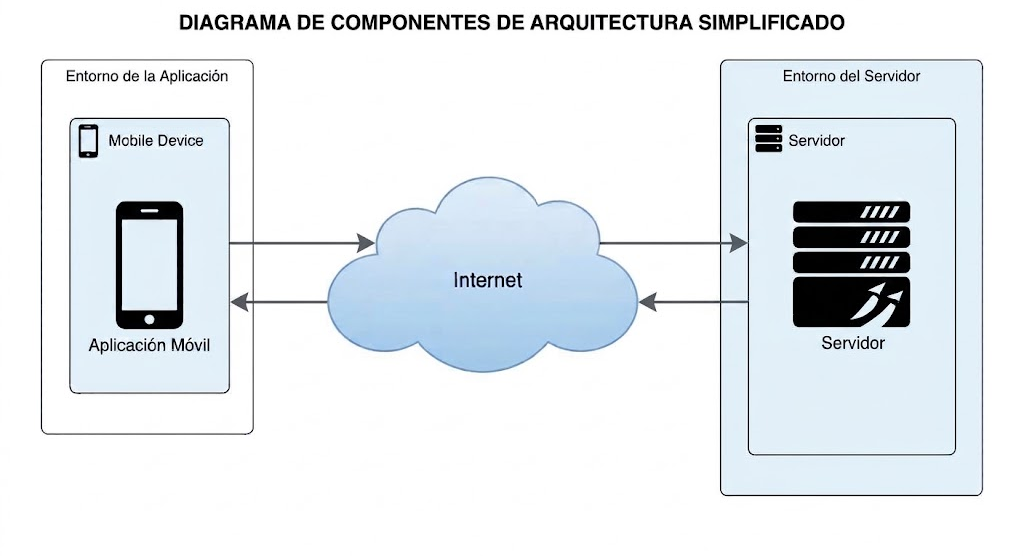
\includegraphics[width=\dimexpr\textwidth-2\fboxrule\relax,height=0.75\textheight,keepaspectratio]{images/arquitectura.png}}

\subsection{Flujo principal}
Las decisiones funcionales responden al contexto de uso observado y se concretan en los requisitos verificables:

\begin{enumerate}[leftmargin=*]
  \item \textbf{Acceso y responsabilidades.} Cada perfil accede solo a las funciones y datos que le corresponden; el administrador gestiona las cuentas y asociaciones. Así se separan las responsabilidades del alumnado, el personal y los tutores. (\hyperlink{rf-01}{RF-01}--\hyperlink{rf-06}{RF-06}; \hyperlink{rnf-03}{RNF-03})

  \item \textbf{Planificación.} El personal asigna actividades durante el horario escolar y los tutores autorizados, fuera de él; el personal también puede asignar rutinas existentes. El alumnado puede añadir actividades personales, diferenciadas de las asignadas. Esta división refleja los distintos roles de apoyo contemplados en los requisitos. (\hyperlink{rf-07}{RF-07}, \hyperlink{rf-10}{RF-10}, \hyperlink{rf-12}{RF-12}, \hyperlink{rf-17}{RF-17}--\hyperlink{rf-19}{RF-19})

  \item \textbf{Consulta accesible.} El alumnado consulta las actividades por fecha y hora, y recibe instrucciones ordenadas con los apoyos configurados para su perfil. La agenda estructurada y los apoyos seleccionables son una respuesta a la necesidad de adaptar la interacción a la dinámica y diversidad del aula; su formato concreto se validará con usuarios. (\hyperlink{rf-20}{RF-20}--\hyperlink{rf-23}{RF-23}; \hyperlink{rnf-01}{RNF-01}, \hyperlink{rnf-05}{RNF-05}, \hyperlink{rnf-06}{RNF-06})

  \item \textbf{Realización y continuidad.} El alumnado completa las instrucciones paso a paso y consulta el progreso; el temporizador acompaña la actividad. Si no hay conexión, conserva el acceso a las actividades sincronizadas y registra el avance para sincronizarlo después. Estas funciones buscan apoyar el seguimiento sin depender de la supervisión continua del personal, sujeto a validación de uso. (\hyperlink{rf-24}{RF-24}--\hyperlink{rf-29}{RF-29}; \hyperlink{rnf-04}{RNF-04}, \hyperlink{rnf-07}{RNF-07})

\end{enumerate}

\end{cambiocontenido}
% ==============================================================================
% SECCIÓN 8: ACTIVIDADES Y CRONOGRAMA
% ==============================================================================

\newpage
\section{Actividades y Cronograma}

Las actividades del proyecto se vinculan a los objetivos específicos definidos en el apartado 2 y se desarrollan mediante una metodología ágil. Tras una fase inicial de análisis y especificación de requisitos, que concluye con la entrega del 22/10/2026, el diseño, la implementación y las pruebas se realizan en tres iteraciones, cada una con su entrega, revisión y retrospectiva (RI-03, RI-04, RI-06). Las fechas de cada iteración coinciden con las entregas previstas en el apartado 10, y la planificación detallada de tareas y su seguimiento se registran en JIRA. Los responsables se asignan según los roles del equipo, y la participación del centro se canaliza a través de los cauces descritos en el apartado 8. Cualquier cambio en las fechas o en el reparto de requisitos entre iteraciones se registrará y comunicará al centro.

\subsection{Actividades y entregables previstos}
\begin{center}
\small
\begin{tabularx}{\textwidth}{|>{\raggedright\arraybackslash}p{2.5cm}|>{\raggedright\arraybackslash}p{1.5cm}|>{\raggedright\arraybackslash}X|>{\raggedright\arraybackslash}p{3.4cm}|}
\hline
\rowcolor{tableHeader}
Actividad & Objetivo & Participantes e implicación & Entregable / evidencia \\
\hline
Fase inicial: análisis y especificación & OBJ-01 & Equipo: Coordinador (lidera) y Catalogador (requisitos y backlog). Centro: exposición inicial (25/09), visita al centro (02/10) y dudas por correo. & Requisitos y alcance aprobados (DC-01) \\
\hline
Diseño de flujos y prototipo & OBJ-02 & Equipo: Gestor de Accesibilidad (lidera) y [quien haga Figma]. Centro y usuarios: revisión del prototipo. & Prototipo y observaciones registradas (DC-02) \\
\hline
Implementación del MVP & OBJ-03 & Equipo: [desarrolladores backend y Flutter]. Centro: resolución de dudas. & Versión con requisitos aprobados al final de cada iteración \\
\hline
Pruebas y ajustes & OBJ-04 & Equipo: Gestor de Calidad (lidera). Centro y usuarios: [validación que se acuerde]. & Informe de pruebas e incidencias (DC-03, DC-05) \\
\hline
Documentación y entrega & OBJ-05 & Equipo: Catalogador (manual) y Presentador (presentación final). Centro: revisión y recepción. & Aplicación y documentación final (DC-04, DC-06) \\
\hline
\end{tabularx}
\end{center}

\subsection{Cronograma}
La planificación visual del anexo abarca de octubre a diciembre y se organiza en cuatro sprints (siendo el 0 el sprint actual). La gestión de usuarios y autenticación se sitúa al inicio, la agenda y la gestión de tareas se desarrollan entre los primeros sprints, los pasos de las actividades y los ajustes de accesibilidad se concentran en la parte intermedia y las tareas alternativas aparecen en el último sprint.
% ==============================================================================
% SECCIÓN 9: CAUCES DE SEGUIMIENTO CON EL CLIENTE
% ==============================================================================
\newpage
\section{Cauces de Seguimiento con el Cliente}


\begin{center}
\small
\begin{tabularx}{\textwidth}{|>{\raggedright\arraybackslash}p{3cm}|>{\raggedright\arraybackslash}p{2.6cm}|>{\raggedright\arraybackslash}X|>{\raggedright\arraybackslash}p{3cm}|}
\hline
\rowcolor{tableHeader}
Cauce propuesto & Frecuencia & Información / propósito & Participación del cliente \\
\hline
Resumen de estado por correo electrónico & Semanal & Trabajo completado, siguiente paso, bloqueos, riesgos y decisiones necesarias. & Nombrar contacto destinatario y responder a decisiones solicitadas. \\
\hline
Reunión de seguimiento & Cada dos semanas & Revisar avances, mostrar el prototipo o versión disponible, resolver dudas y acordar cambios. & Asistir con el interlocutor designado y validar acuerdos. \\
\hline
Registro compartido de decisiones e incidencias & Actualización continua & Mantener identificador, descripción, impacto, responsable y estado de cada decisión o incidencia. & Revisar y confirmar las decisiones que requieran aprobación del centro. \\
\hline
Reunión de inicio con el centro (realizada el 25/09/2026, en la ETSIIT) & Una vez, al inicio & Exposición en clase sobre el centro, el alumnado PTVAL y la necesidad que origina la app; sesión de preguntas y respuestas con el alumnado de la asignatura. Origen de los requisitos iniciales. & El tutor y la profesora del centro presentaron la necesidad y resolvieron las dudas planteadas. \\
\hline
Visita al centro (realizada el 02/10/2026 por nuestro compañero de grupo) & Una visita realizada & Conocer el contexto real: espacios, dinámica de las clases, apoyos que ya utilizan y forma de trabajar con el alumnado. Contrastar los requisitos con la realidad del centro. & Recibir al miembro del equipo y mostrar el centro y su funcionamiento. \\
\hline
Material del centro en PRADO & Consulta continua & Documentación aportada por el centro como referencia para requisitos y apoyos visuales. & Aportar material adicional si lo considera útil. \\
\hline
Orientación del profesorado de DGP y MDA & Sesiones de clase y tutorías & Orientación sobre el enfoque del proyecto y la documentación. No sustituye las decisiones del centro. & Ninguna (cauce interno académico). \\
\hline
\end{tabularx}
\end{center}

El equipo enviará un aviso extraordinario cuando una incidencia pueda afectar a un requisito aprobado, una fecha objetivo o la seguridad de los datos. Se registrará la decisión del centro en el acta o registro correspondiente; los cambios de alcance no se darán por aprobados solo por comunicarlos en el informe de estado.
% ==============================================================================
% SECCIÓN 10: VALOR AÑADIDO, BENEFICIOS Y BENEFICIARIOS
% ==============================================================================
\newpage
\section{Valor Añadido, Beneficios y Beneficiarios}

\subsection{Valor añadido de la propuesta}
Frente a las agendas visuales estáticas o diarios tradicionales analizados en el estudio previo (como \textit{In-TIC Agenda} o \textit{Día a Día}), \textbf{AUTOVIDA} incorpora capacidades orientadas a la autonomía activa, la gestión de imprevistos y la continuidad entre el aula y el entorno familiar:

\begin{center}
\small
\begin{tabularx}{\textwidth}{|>{\raggedright\arraybackslash}p{3.5cm}|>{\raggedright\arraybackslash}X|>{\raggedright\arraybackslash}p{3.2cm}|}
\hline
\rowcolor{tableHeader}
\textbf{Elemento diferenciador} & \textbf{Valor que aporta al centro y a los usuarios} & \textbf{Trazabilidad} \\
\hline
Gestión de imprevistos y actividades alternativas & Permite asociar una actividad de respaldo cuando la principal no puede completarse y reajustar la planificación si una tarea se prolonga, reduciendo el bloqueo o la frustración del alumnado ante cambios de rutina. & RF-13, RF-34 a RF-36 y Flujo principal \\
\hline
Iniciativa propia con control de prioridad & El alumnado puede crear sus propias tareas personales para fomentar su autogestión, pero el sistema garantiza que tengan prioridad inferior para no solapar ni desplazar la planificación docente. & RF-17 a RF-19 \\
\hline
Coordinación por franjas horarias (Centro--Hogar) & Delimita automáticamente los permisos de asignación según el horario: el personal gestiona la jornada escolar y los tutores/familias el horario extraescolar, unificando la agenda sin conflictos de edición. & RF-07, RF-10 y RF-20 \\
\hline
Continuidad sin conexión (\textit{Offline-first}) & Permite al alumnado consultar su agenda previamente sincronizada y marcar pasos completados sin depender de la cobertura de red en cada aula, sincronizando el avance al recuperar la conexión. & RNF (Funcionamiento sin conexión y Consistencia) \\
\hline
Seguimiento granular y alertas de cierre diario & Sustituye la revisión manual presencial por el registro paso a paso (obligatorio o guiado), temporizador pausable y notificaciones automáticas al final del día sobre tareas no completadas. & RF-22, RF-24 a RF-29 \\
\hline
Avisos ante cambios relevantes del alumno & Notifica a tutores y personal autorizados cuando se produzcan cambios en los datos, los apoyos o la planificación de un alumno que requieran su atención, facilitando una respuesta coordinada y evitando avisos innecesarios. & RF-41 \\
\hline
\end{tabularx}
\end{center}

\begin{cambiocontenido}{cambioBeneficios}
\subsection{Beneficios y beneficiarios}
Los beneficios esperados se distribuyen entre quienes utilizarán AUTOVIDA de forma directa y quienes pueden beneficiarse de una mejor coordinación educativa. Su alcance dependerá de los perfiles que el centro autorice, de la validación del MVP y de la incorporación de la herramienta a la dinámica habitual. La aplicación se plantea como apoyo a la intervención educativa y familiar, no como sustituto del acompañamiento personal ni del criterio profesional.

\begin{small}
\begin{longtable}{|>{\raggedright\arraybackslash}p{3.2cm}|>{\raggedright\arraybackslash}p{2.4cm}|>{\raggedright\arraybackslash}p{9.6cm}|}
\hline
\rowcolor{tableHeader}
\textbf{Beneficiario} & \textbf{Alcance previsto} & \textbf{Beneficio esperado y método de verificación} \\
\hline
\endfirsthead
\hline
\rowcolor{tableHeader}
\textbf{Beneficiario} & \textbf{Alcance previsto} & \textbf{Beneficio esperado y método de verificación} \\
\hline
\endhead
Alumnado de PTVAL (\textit{beneficiario directo y principal}) & Alumnado de las aulas PTVAL seleccionadas que participe en la validación. & \textbf{Beneficio:} Disponer de una agenda diaria más previsible y comprensible, consultar actividades con apoyos ajustados a cada perfil (texto, pictogramas, imágenes o recursos audiovisuales) y avanzar por instrucciones paso a paso. Las actividades alternativas y el registro del progreso pueden facilitar la gestión de cambios y favorecer una participación más autónoma, siempre con el acompañamiento que cada alumno necesite.\newline \textbf{Verificación:} Pruebas de aceptación y usabilidad acordadas con el centro: observar si los participantes localizan su actividad, comprenden los apoyos, marcan instrucciones, usan el temporizador y consultan una actividad alternativa; registrar dificultades y necesidades de apoyo (RF-13, RF-20 a RF-28; RNF-01, RNF-05 y RNF-06). \\
\hline
Profesorado (\textit{beneficiario directo}) & Docentes autorizados que planifican actividades y rutinas para el alumnado asociado. & \textbf{Beneficio:} Organizar las actividades escolares en un único espacio, reutilizar rutinas y consultar el avance registrado para preparar apoyos o ajustes posteriores. La asignación por horario y las alertas de cierre pueden facilitar el seguimiento, sin presuponer que reduzcan por sí solas el tiempo de preparación o supervisión.\newline \textbf{Verificación:} Completar escenarios de creación y asignación de actividades dentro del horario escolar, asignación de rutinas, consulta del progreso y recepción de avisos de tareas pendientes; recoger incidencias y valoración del profesorado (RF-10, RF-12, RF-22 a RF-29). \\
\hline
Personal de apoyo educativo (\textit{beneficiario directo}) & Profesionales autorizados que acompañan al alumnado durante la jornada y tienen alumnos asociados. & \textbf{Beneficio:} Consultar las actividades y apoyos previstos, registrar el progreso observado y coordinar la atención con el profesorado y los tutores autorizados. Esto puede ayudar a mantener una referencia común sobre la tarea en curso y los cambios planificados.\newline \textbf{Verificación:} Probar con cuentas autorizadas la consulta de alumnos asociados, el acceso a sus actividades, el registro del progreso y la recepción de notificaciones; comprobar también que no se accede a información de alumnos no asociados (RF-11, RF-22 a RF-29 y RNF-03). \\
\hline
Tutores legales y familias (\textit{beneficiarios directos y secundarios}) & Familias autorizadas vinculadas al alumnado participante. & \textbf{Beneficio:} Consultar y, dentro de los permisos y horarios definidos, organizar actividades del entorno extraescolar con apoyos coherentes con los utilizados en el centro. Las notificaciones sobre tareas pendientes o cambios relevantes pueden facilitar el seguimiento y la comunicación, sin convertir la aplicación en un canal de supervisión permanente.\newline \textbf{Verificación:} Comprobar la asignación y modificación de actividades fuera del horario escolar, la consulta de alumnos asociados y la recepción de avisos pertinentes; confirmar que usuarios no autorizados no acceden a los datos (RF-07 a RF-09, RF-11, RF-29 y RF-41; RNF-03). \\
\hline
Orientación y coordinación pedagógica (\textit{beneficiarios indirectos, si participan}) & Profesionales que colaboren en la definición de apoyos y en la validación acordada con el centro. & \textbf{Beneficio:} Contar con un recurso común para revisar si la presentación de actividades y los apoyos configurados resultan adecuados para las necesidades observadas, e identificar aspectos que convenga ajustar. AUTOVIDA no realiza diagnósticos ni sustituye la valoración profesional.\newline \textbf{Verificación:} Revisar con estos perfiles los ajustes de accesibilidad y los escenarios de uso, documentar observaciones y comprobar que los cambios acordados se reflejan en la configuración validada (RF-37, cuyo alcance está pospuesto, y RNF-01, RNF-05 y RNF-06). \\
\hline
Administración del sistema (\textit{beneficiario operativo}) & Personas designadas por el centro para gestionar las cuentas de alumnado, tutores y personal. & \textbf{Beneficio:} Disponer de operaciones centralizadas para crear, consultar, modificar y eliminar cuentas, facilitando la organización inicial de usuarios y el mantenimiento de la información básica del sistema.\newline \textbf{Verificación:} Ejecutar los casos de prueba de gestión de cuentas para cada tipo de usuario y comprobar que los cambios se reflejan correctamente y que se respetan los permisos definidos (RF-30 a RF-33 y RNF-03). \\
\hline
C.E.E. Fundación Purísima Concepción (\textit{beneficiario institucional}) & Comunidad educativa y responsables del programa PTVAL del centro. & \textbf{Beneficio:} Participar en la definición y validación de una solución ajustada a sus necesidades, disponer de documentación del producto y valorar su utilidad antes de decidir si se integra en sus procesos. Su sostenibilidad dependerá de los recursos de mantenimiento, soporte y protección de datos que se acuerden.\newline \textbf{Verificación:} Revisar y aceptar, según los criterios acordados, el MVP, la guía de uso y el informe de pruebas; registrar decisiones, limitaciones y propuestas de mejora al cierre de las iteraciones previstas (OBJ-04 y OBJ-05). \\
\hline
Futuras promociones de PTVAL (\textit{beneficiarios potenciales indirectos}) & Alumnado y profesionales que podrían utilizar la solución en cursos posteriores, si el centro decide mantenerla. & \textbf{Beneficio:} Aprovechar las lecciones aprendidas durante el piloto y, si se confirma la adecuación de la herramienta, contar con una base reutilizable que pueda adaptarse a nuevos perfiles y necesidades. Este beneficio no se considera alcanzado hasta que el centro valide la solución y acuerde su continuidad.\newline \textbf{Verificación:} Evaluar los resultados del piloto, documentar mejoras pendientes y comprobar si existe una decisión del centro sobre mantenimiento, adaptación y uso en cursos posteriores. \\
\hline
Equipo del proyecto y comunidad universitaria (\textit{beneficiarios académicos indirectos}) & Estudiantes y docentes que participan en el proyecto de Aprendizaje-Servicio. & \textbf{Beneficio:} Aplicar conocimientos de ingeniería del software, accesibilidad, gestión de requisitos y validación en colaboración con una entidad real, incorporando la retroalimentación del centro al trabajo académico.\newline \textbf{Verificación:} Revisar la trazabilidad entre necesidades, requisitos, prototipo y pruebas, así como las actas, entregables y reflexiones del proyecto. \\
\hline
\end{longtable}
\end{small}

El número exacto de cuentas y perfiles activos se acordará con la dirección del centro al inicio de la primera iteración. Para valorar los beneficios sin dar por logrados resultados que aún deben comprobarse, se establecerá una línea base y se compararán los resultados de las pruebas de validación. Entre los indicadores posibles se encuentran la proporción de actividades completadas con distintos niveles de apoyo, la identificación de actividades por parte del alumnado, el tiempo necesario para preparar una rutina y la valoración de familias y profesionales sobre la continuidad entre centro y hogar. La recogida de estos datos deberá acordarse con el centro, respetar la privacidad del alumnado y considerar el tamaño y las características de la muestra.
\end{cambiocontenido}

% ==============================================================================
% SECCIÓN 11: DOCUMENTACIÓN Y ACTAS
% ==============================================================================
\newpage
\section{Documentación para el Cliente y Actas del Proyecto}

Se mantendrán dos conjuntos diferenciados: documentación preparada para la entidad destinataria y registros internos del equipo. Los documentos previstos se ajustarán al alcance finalmente aprobado y se entregarán en los formatos y fechas que se acuerden.

\subsection{Documentación propuesta para el cliente}
\begin{center}
\small
\begin{tabularx}{\textwidth}{|>{\raggedright\arraybackslash}p{1cm}|>{\raggedright\arraybackslash}p{3.2cm}|>{\raggedright\arraybackslash}X|>{\raggedright\arraybackslash}p{2cm}|>{\raggedright\arraybackslash}p{2.6cm}|}
\hline
\rowcolor{tableHeader}
ID & Documento & Contenido previsto & Responsable & Fecha objetivo \\
\hline
DC-01 & Propuesta técnica y Especificación de requisitos & Requisitos identificados, prioridades, criterios de aceptación, exclusiones y cambios acordados. & Coordinador & 22/10/2026 \\
\hline
DC-02 & Documentos de análisis, diseño y arquitectura & Diagramas UML, diagrama entidad-relación (E/R), diseño de interfaz y descripción de la arquitectura del sistema y sus componentes. & Coordinador & 12/11/2026, \newline 03/12/2026, \newline 21/12/2026 \\
\hline
DC-03 & Informes de pruebas y gestión de calidad & Pruebas ejecutadas, resultados, incidencias conocidas y justificación de la calidad del producto y proceso. & Gestor de calidad & 12/11/2026, \newline 03/12/2026, \newline 21/12/2026 \\
\hline
DC-04 & Manual de usuario (Opcional) & Instrucciones para el personal y el alumnado sobre las funciones que se incluyan en la versión entregada. & Catalogador & 21/12/2026 \\
\hline
DC-05 & Informe de usabilidad-accesibilidad & Auditoría de cumplimiento de normativas de accesibilidad y adaptación de la interfaz a los perfiles NEAE. & Gestor de usabilidad y accesibilidad & 21/12/2026 \\
\hline
DC-06 & Documento de presentación del proyecto completo & Documento resumen y material de apoyo para la presentación final del proyecto ante el cliente. & Presentador & 12/01/2027 \\
\hline
\end{tabularx}
\end{center}

\subsection{Registros internos del equipo y gestión del proyecto}
Además de la documentación orientada al cliente, el equipo elaborará y mantendrá una serie de registros internos y documentos de gestión exigidos para el seguimiento académico y la evaluación del proyecto. Estos documentos reflejan la planificación, el control de calidad, los recursos y la metodología ágil aplicada.

\begin{center}
\small
\begin{tabularx}{\textwidth}{|>{\raggedright\arraybackslash}p{1cm}|>{\raggedright\arraybackslash}p{3.2cm}|>{\raggedright\arraybackslash}X|>{\raggedright\arraybackslash}p{2cm}|>{\raggedright\arraybackslash}p{2.6cm}|}
\hline
\rowcolor{tableHeader}
ID & Documento & Contenido previsto & Responsable & Fecha objetivo \\
\hline
RI-01 & Manual de coordinación & Normas internas, canales de comunicación, uso del repositorio de control de versiones y reparto inicial de roles. & Coordinador & 22/10/2026 \\
\hline
RI-02 & Presupuesto justificado & Estimación de costes asociados al desarrollo del proyecto, recursos humanos y herramientas. & Coordinador & 22/10/2026 \\
\hline
RI-03 & Planificación y documentos de gestión & Planificación temporal de cada iteración (inicial y real), gestión de recursos, riesgos, costes y adquisiciones. & Coordinador & 22/10/2026, \newline 12/11/2026, \newline 03/12/2026, \newline 21/12/2026 \\
\hline
RI-04 & Artefactos Ágiles (Backlog y Tablero) & Personajes, escenarios, Product Backlog, plan de entregas e informes de evolución del tablero (JIRA). & Catalogador / Coordinador & 22/10/2026, \newline 12/11/2026, \newline 03/12/2026, \newline 21/12/2026 \\
\hline
RI-05 & Registro de horas dedicadas & Documento con el tiempo dedicado por cada miembro del equipo a las distintas tareas del proyecto. & Todos los miembros & 22/10/2026, \newline 12/11/2026, \newline 03/12/2026, \newline 21/12/2026 \\
\hline
RI-06 & Actas de reuniones e informes de retrospectiva & Registro de decisiones, informes tras reuniones de revisión y retrospectiva de cada iteración. & Moderador & Continua \\
\hline
\end{tabularx}
\end{center}

Los documentos y sus versiones se mantendrán en el repositorio compartido del equipo. El manual de coordinación fijará la frecuencia de actualización y las reglas de revisión.

% ==============================================================================
% ANEXO A: CRONOGRAMA VISUAL
% ==============================================================================

\clearpage
\appendix

\section{Cronograma visual}

\begin{figure}[htbp]
    \centering
    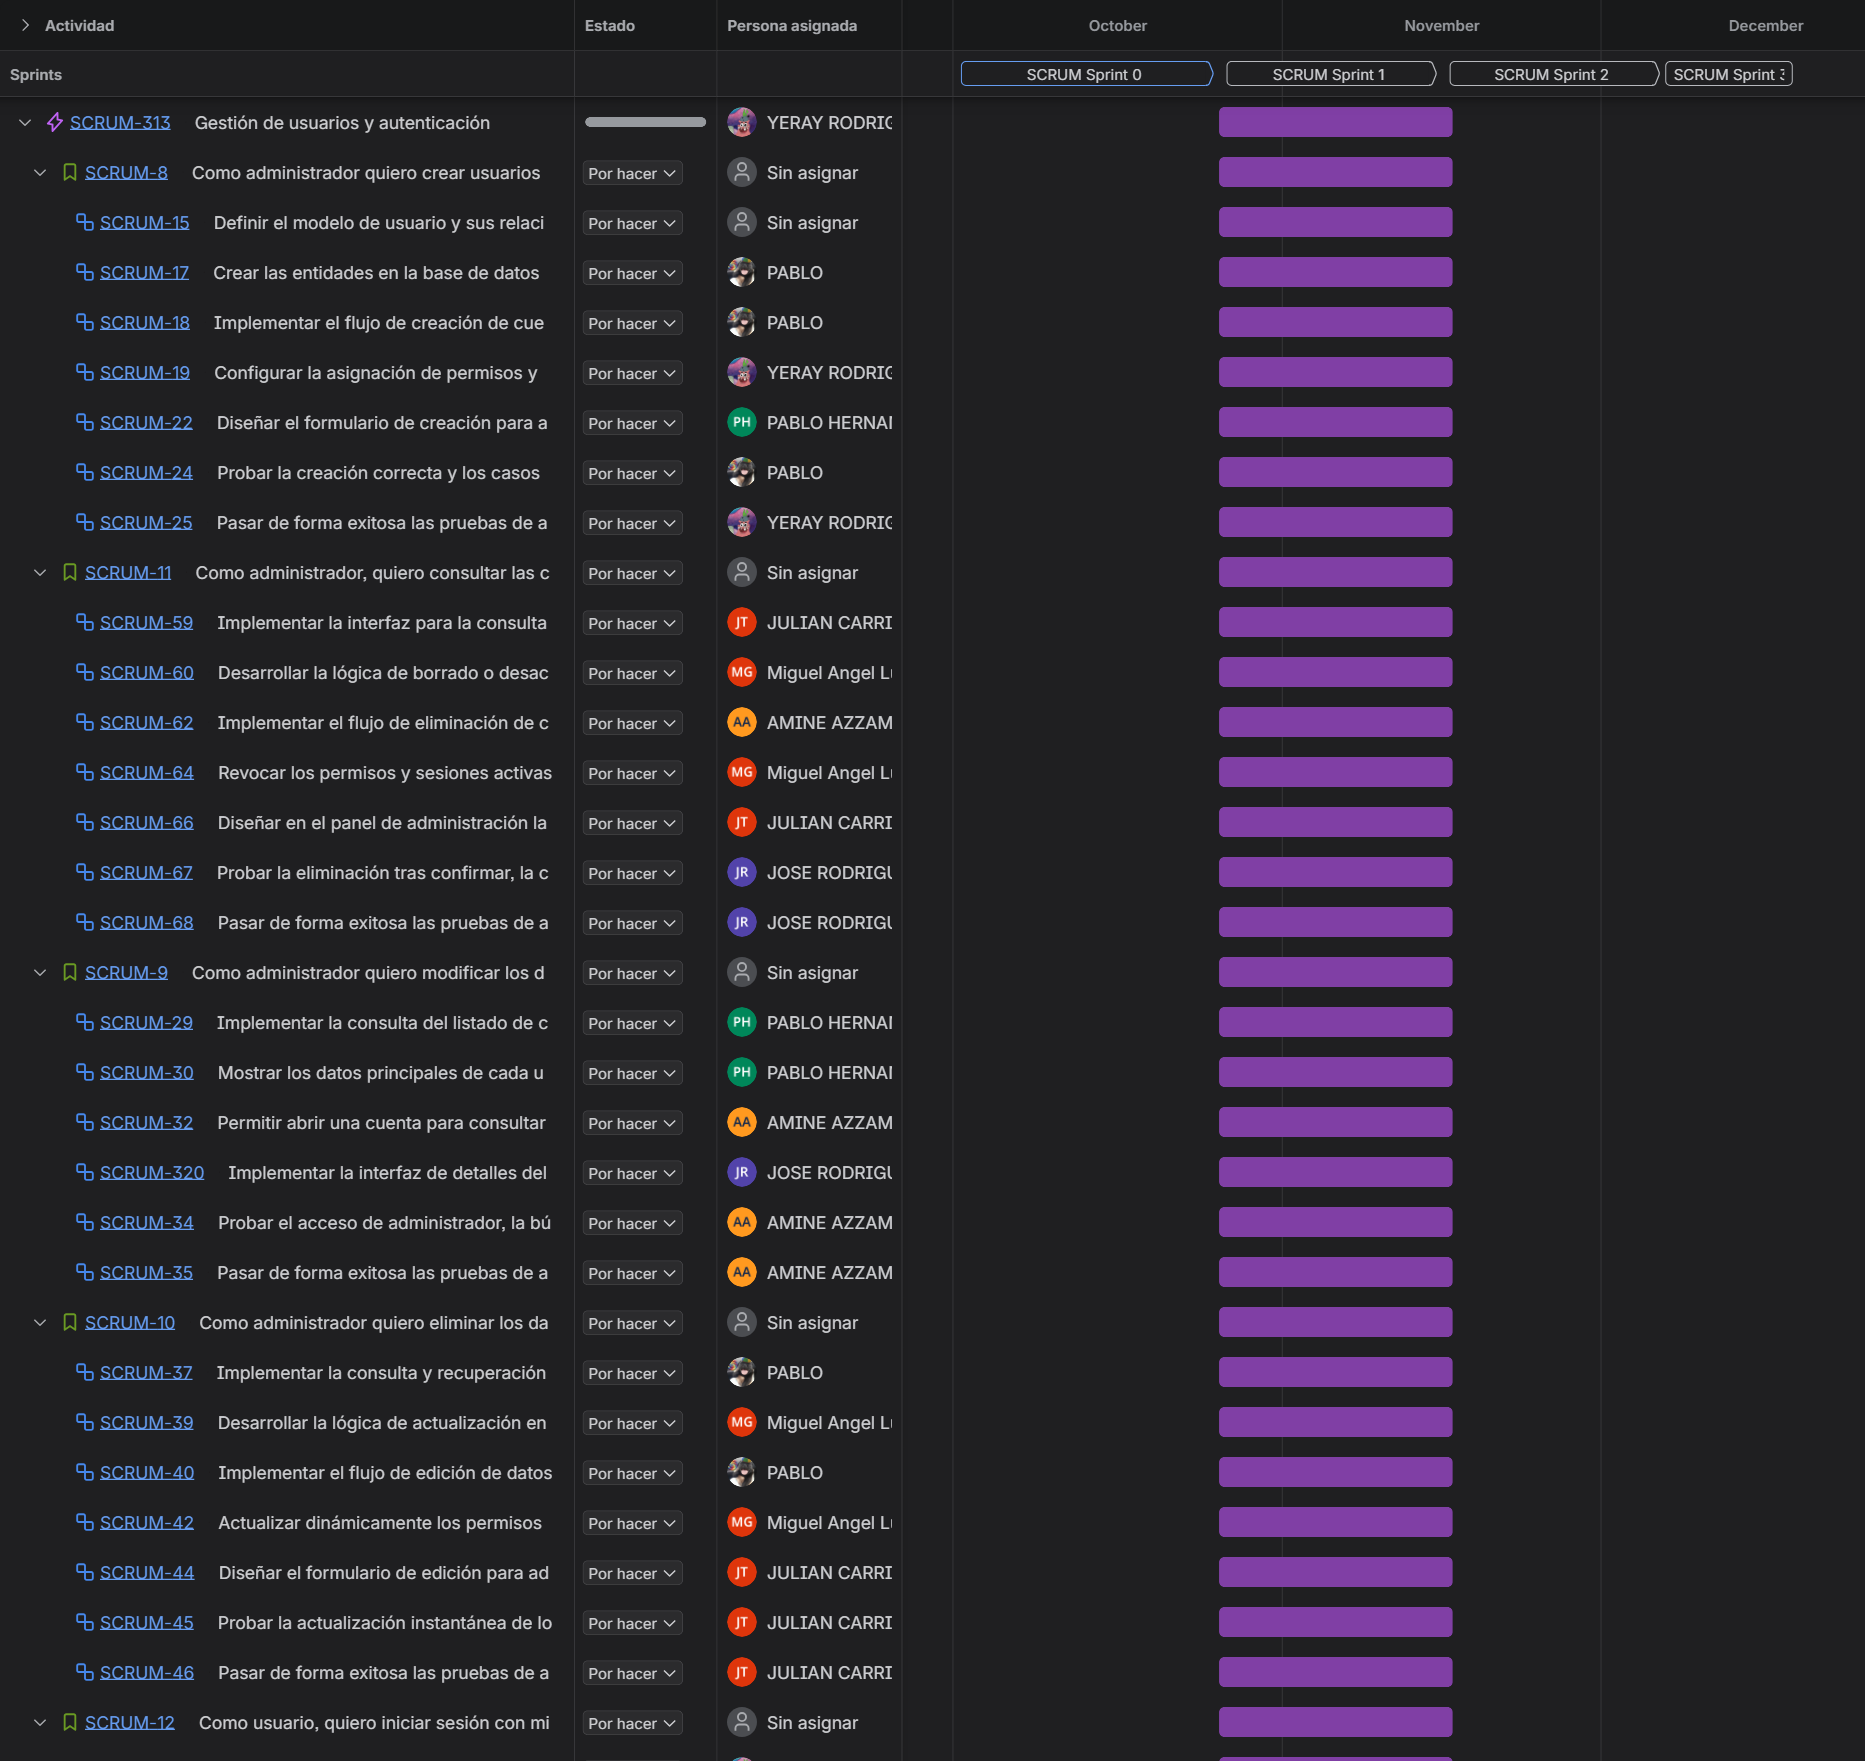
\includegraphics[width=0.95\linewidth]{images/cronograma1.png}
    \caption{Diagrama de Arquitectura (Parte 1)}
    \label{fig:arquitectura_p1}
\end{figure}

\begin{figure}[htbp]
    \centering
    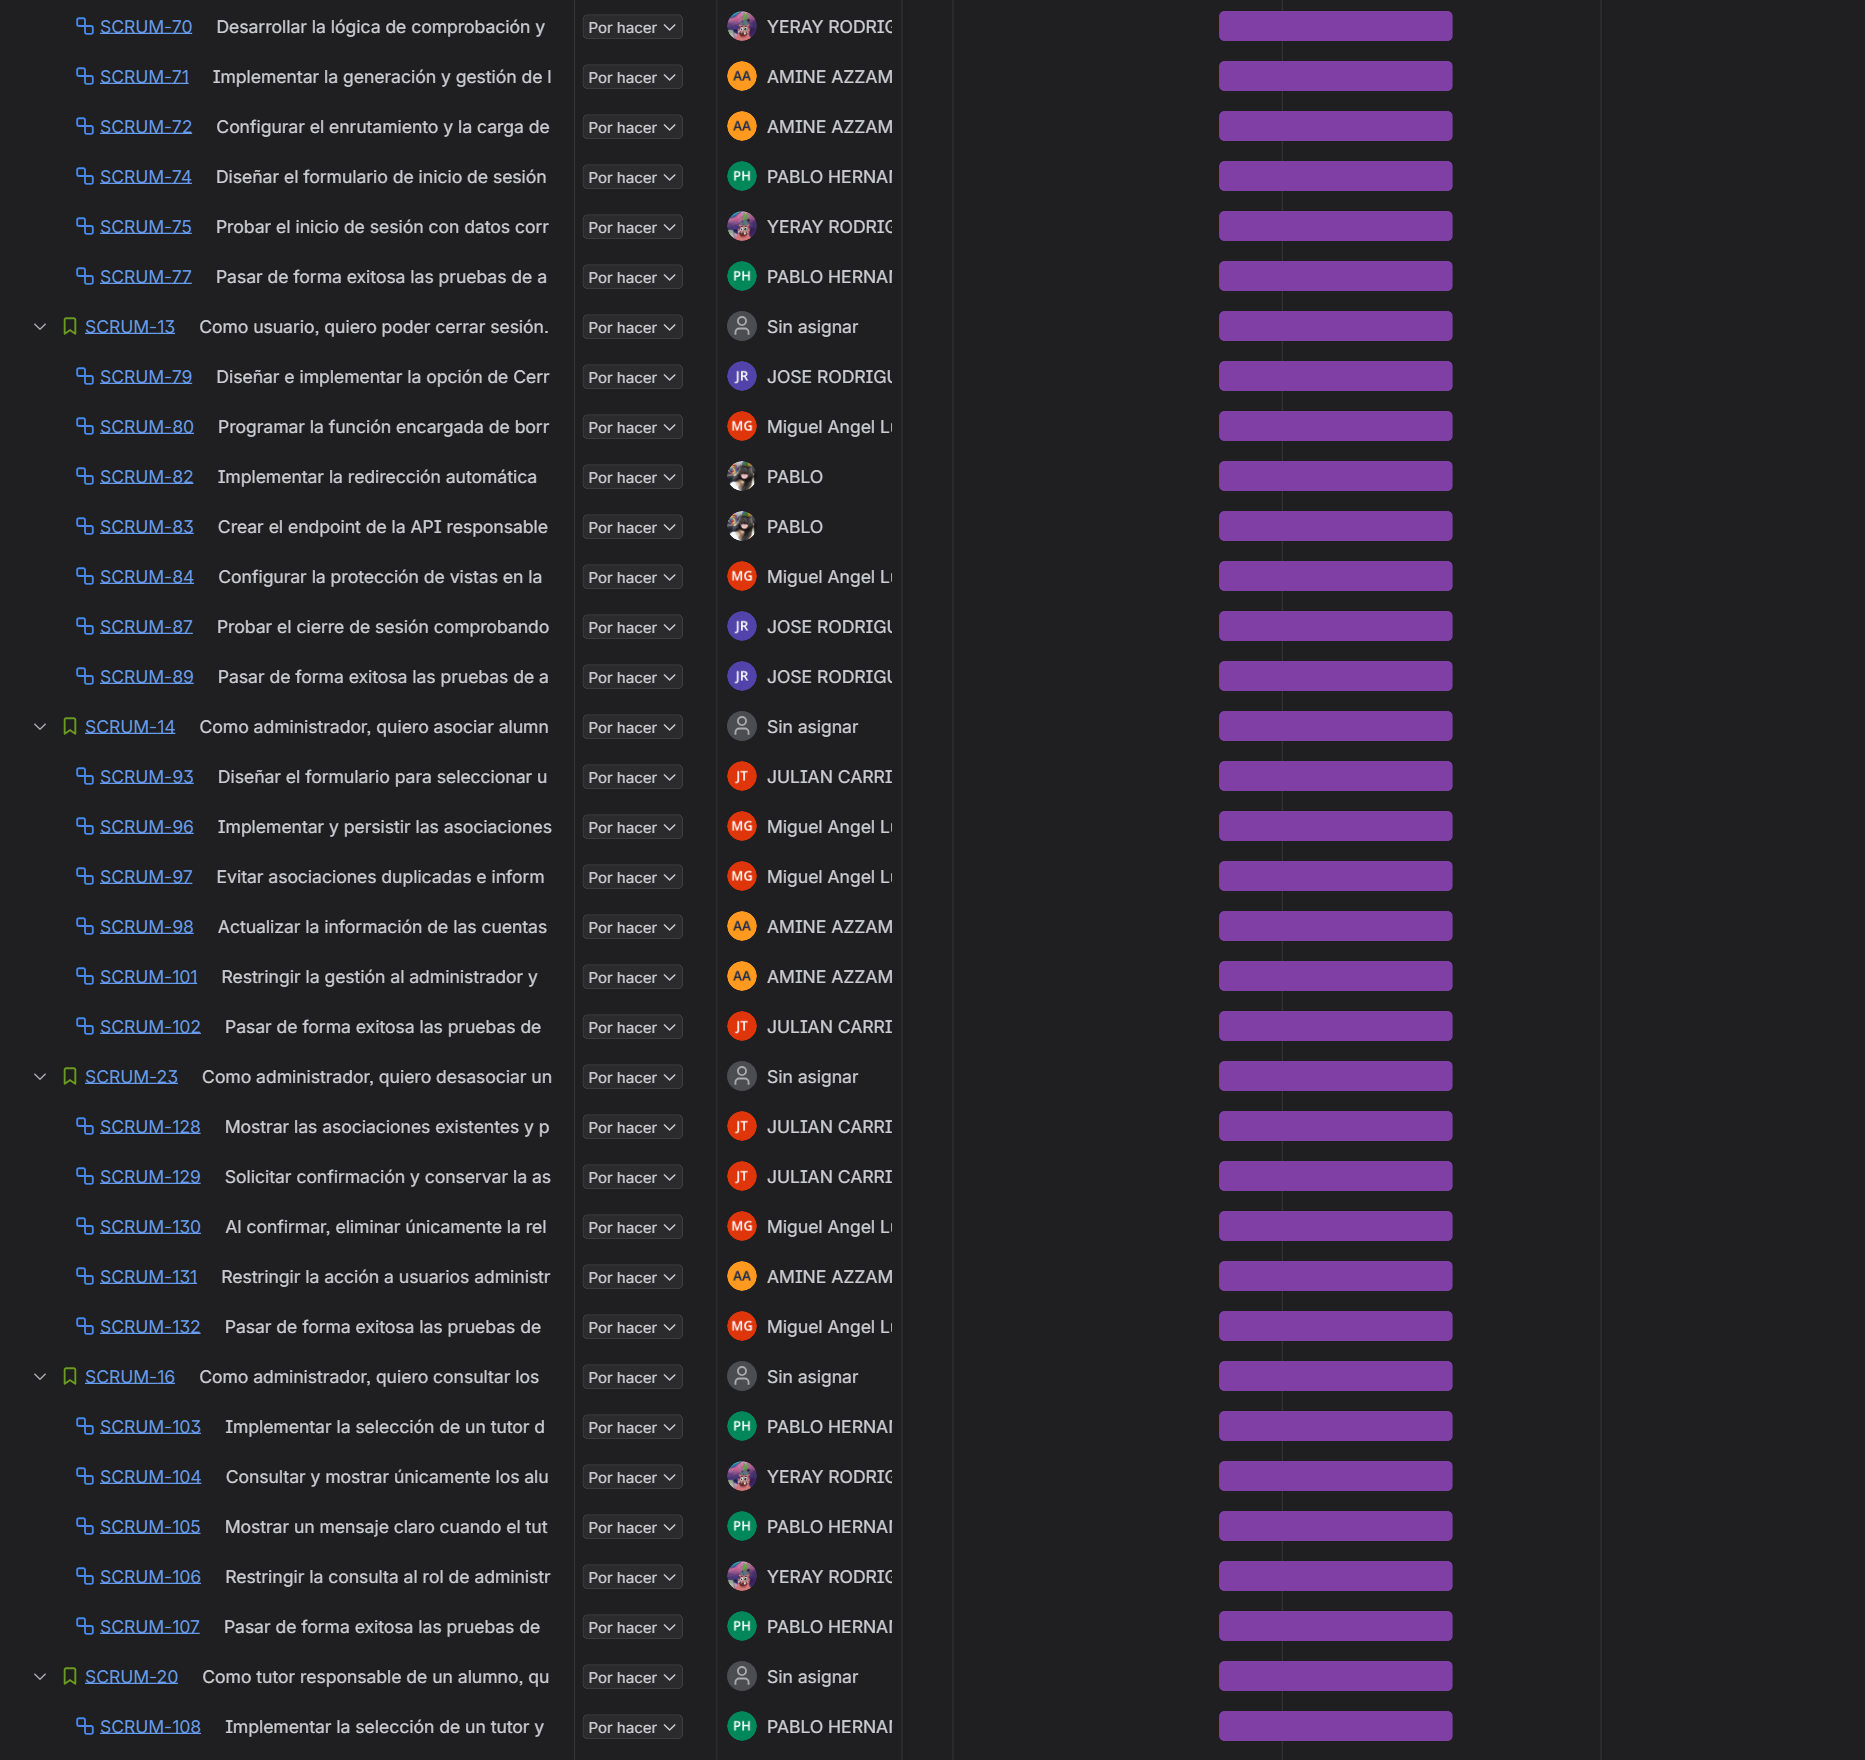
\includegraphics[width=0.95\linewidth]{images/cronograma2.png}
    \caption{Diagrama de Arquitectura (Parte 2)}
    \label{fig:arquitectura_p2}
\end{figure}

\begin{figure}[htbp]
    \centering
    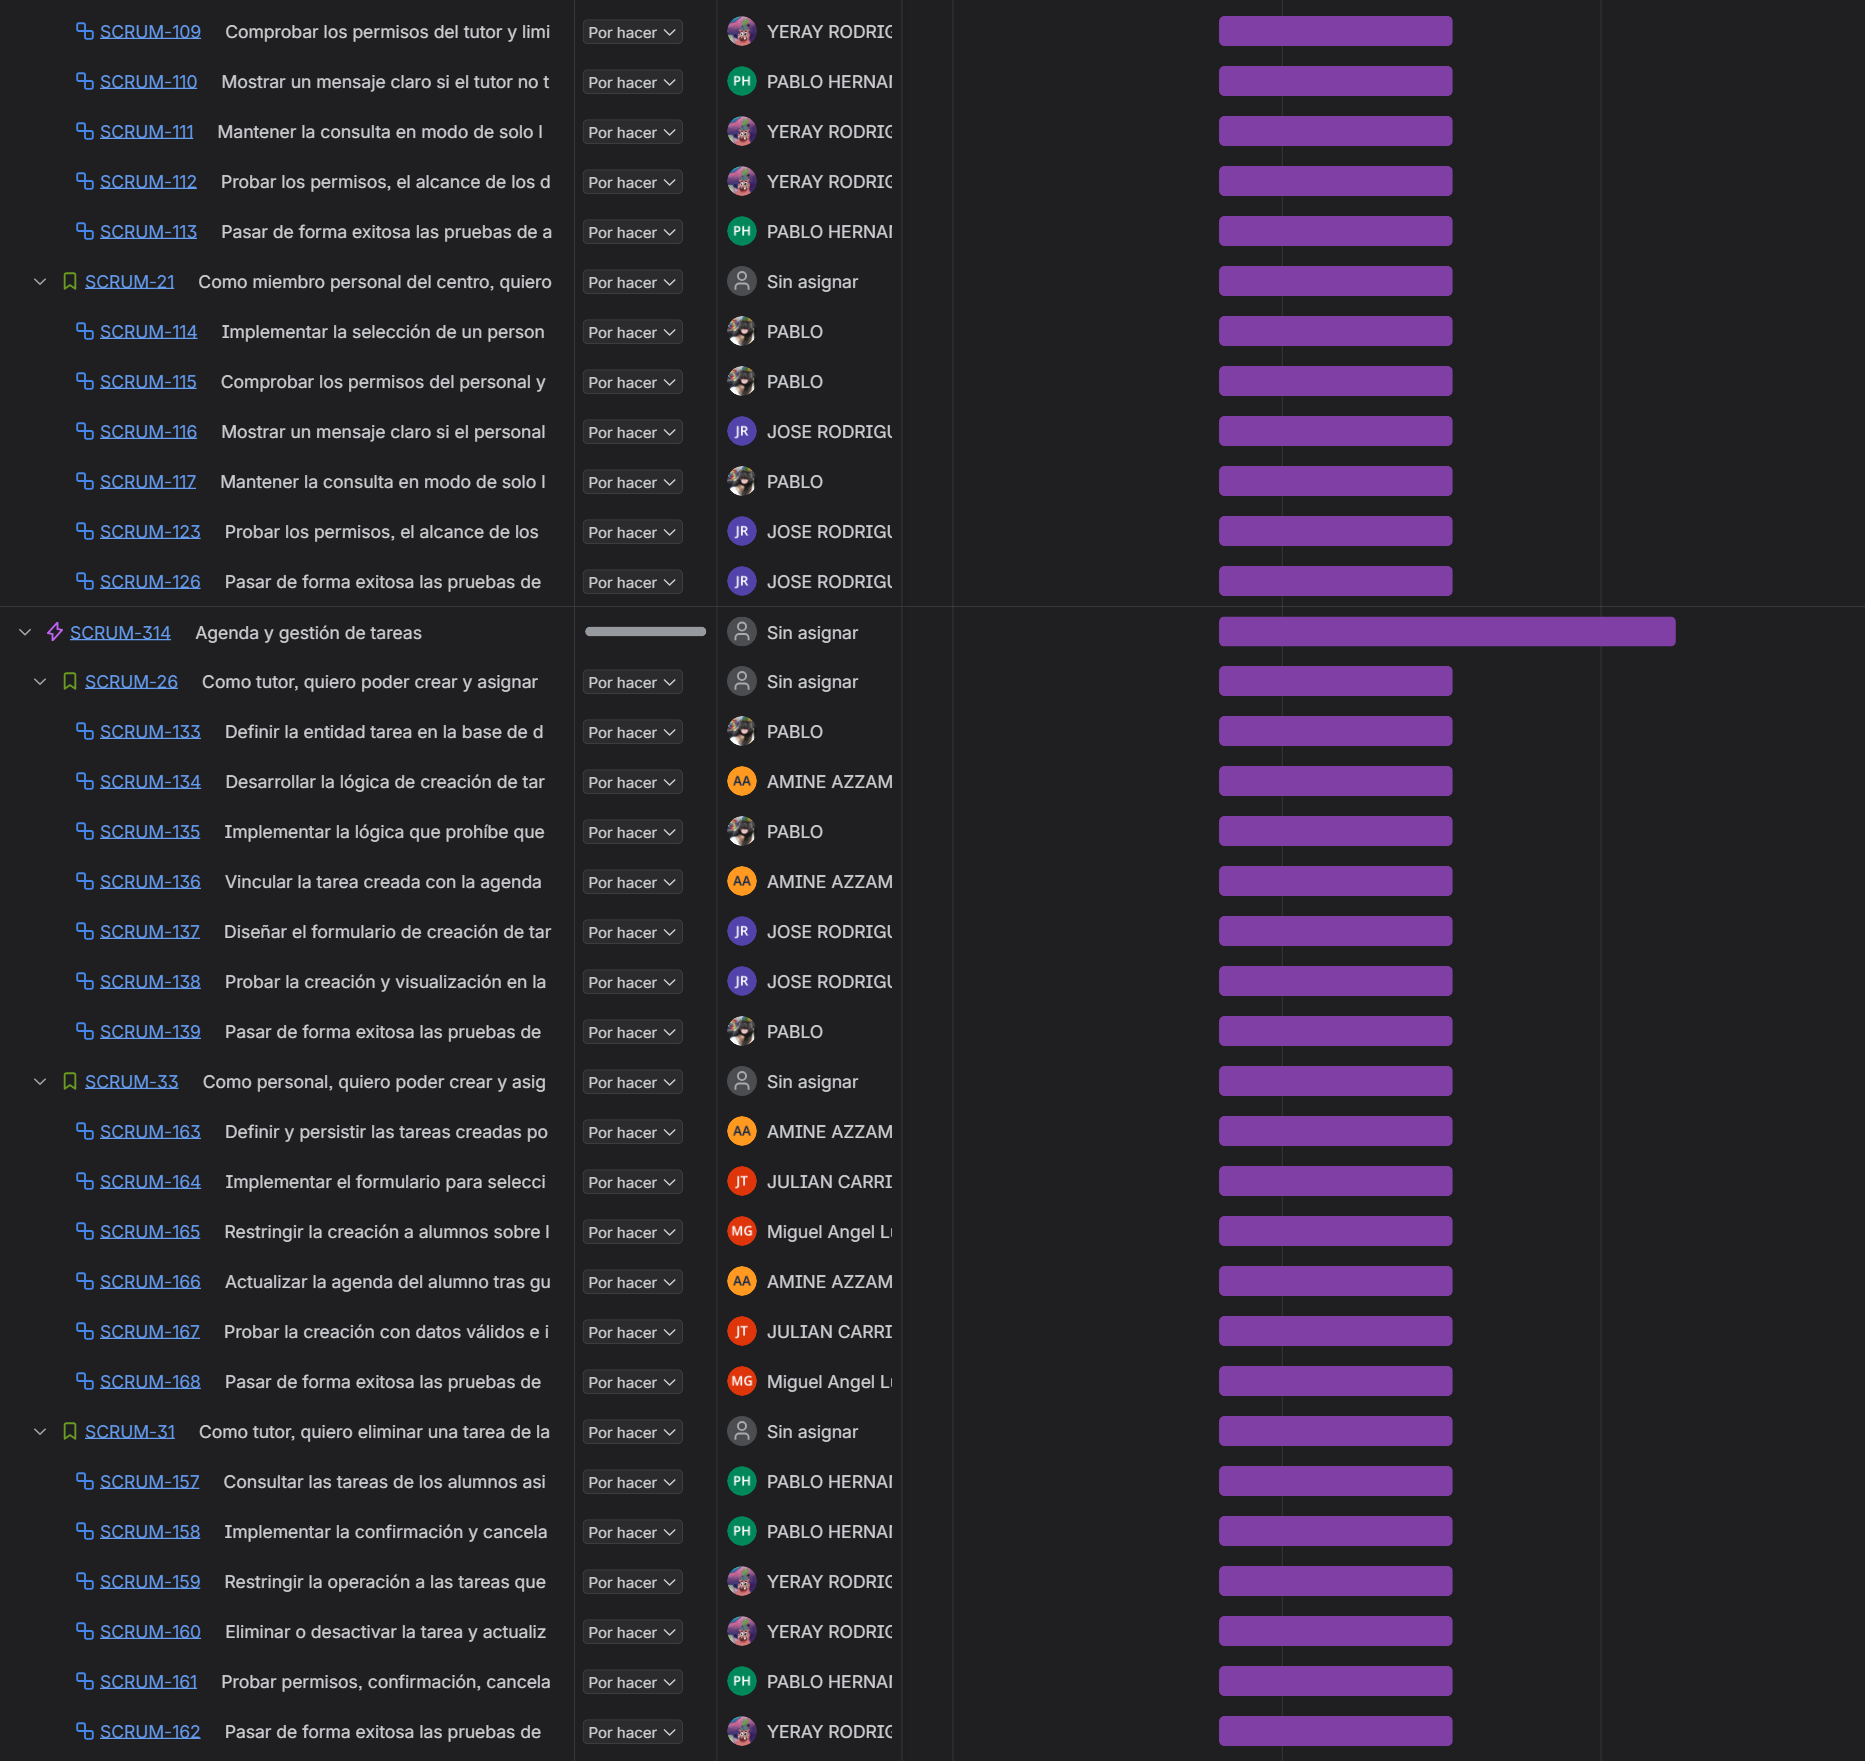
\includegraphics[width=0.95\linewidth]{images/cronograma3.png}
    \caption{Diagrama de Arquitectura (Parte 3)}
    \label{fig:arquitectura_p3}
\end{figure}

\begin{figure}[htbp]
    \centering
    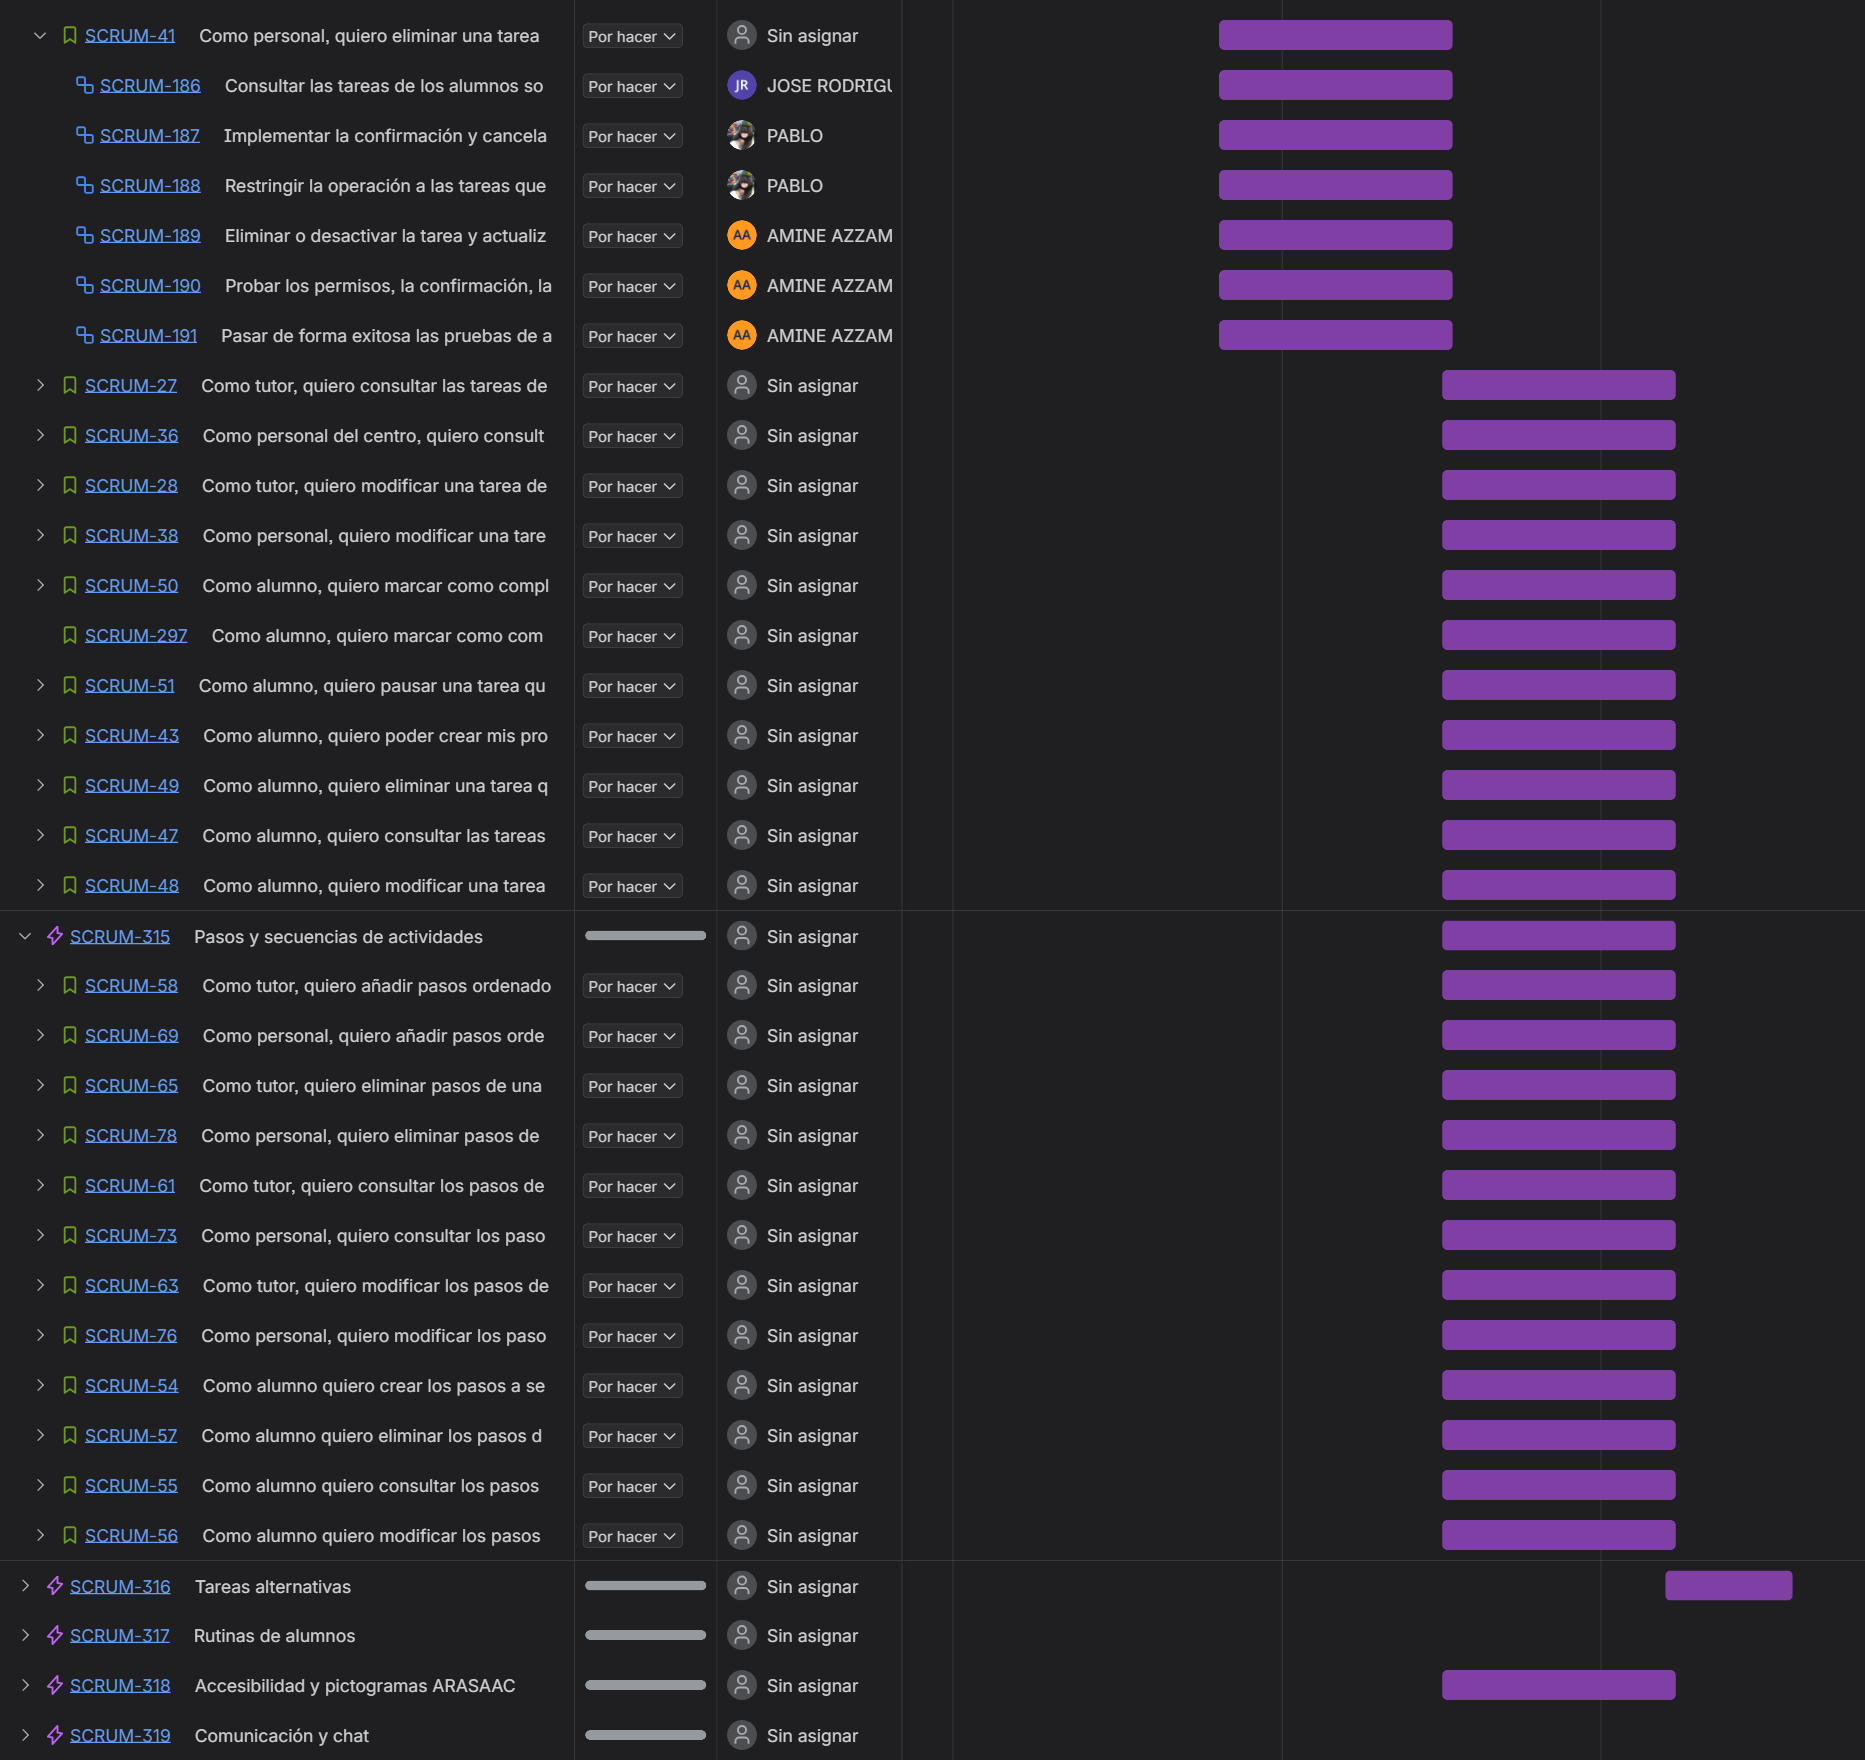
\includegraphics[width=0.95\linewidth]{images/cronograma4.png}
    \caption{Diagrama de Arquitectura (Parte 4)}
    \label{fig:arquitectura_p4}
\end{figure}




\end{document}